\newcommand{\beginsupplementary}{
    \setcounter{section}{0}
	\renewcommand{\thesection}{A\arabic{section}}
	\renewcommand{\thesubsection}{\thesection.\arabic{subsection}}

	\renewcommand{\thetable}{A\arabic{table}}
	\setcounter{table}{0}

	\renewcommand{\thefigure}{A\arabic{figure}}
	\setcounter{figure}{0}
}

\newcommand{\suptitle}{Appendix for:\\ \papertitle}

\newcommand{\maketitlesupp}{
    \vskip .375in
    \begin{center}
        \Large \bf \suptitle \par
    \end{center}
    \vspace{24pt}}
\beginsupplementary
\maketitlesupp

{\noindent The appendix is organized as follows:}
\begin{itemize}
\item In~\secref{sec:supp_anomaly_detection}, we present \textbf{a third application}, GAN-based \textit{One-vs-All} anomaly detection using AR features, and show its benefits over standard techniques.
\item In~\secref{sec:supp_results}, we provide additional experimental results on feature inversion.
\item In~\secref{sec:supp_additional}, we provide additional experimental results on downstream tasks. 
\item In~\secref{sec:supp_proposed_method}, we provide implementation and experimental setup details.
\end{itemize}

\section{Anomaly Detection using AR Representations}
\label{sec:supp_anomaly_detection}
\subsection{Approach}
\textit{One-vs-All} anomaly detection is the task of identifying samples that do not fit an expected pattern \cite{golan_2018_deep,deecke_2018_image,ruff_2019_deep,wang_2019_effective}. Given an unlabeled image dataset with normal (\textit{positives}) and anomalous instances (\textit{negatives}), the goal is to distinguish between them. Following GAN-based techniques \cite{deecke_2018_image}, we train our proposed AR AlexNet autoencoder exclusively on positives to learn a how to accurately reconstruct them. Once trained on such a target distribution, we use its reconstruction accuracy to detect negatives.

Given an unlabeled sample $x$ and its AR features $f$, we search for $\hat{f}$ that yields the best reconstruction $\hat{x}=G_{\tilde{\phi}}(\hat{f})$ based on the following criterion (\figref{fig:proposed_anomaly}):
\begin{align}
    \label{eq:anomaly_detection}
    \hat{f}=\ \text{arg }\underset{f}{\text{min}}&\ \alpha_{\text{pix}}\|G_{\tilde{\phi}}(f)-x\|_{1}+ \alpha_{\text{feat}}\|F_{\tilde{\theta}}\circ G_{\tilde{\phi}}(f)-F_{\tilde{\theta}}(x)\|_{2}^{2},
\end{align}
where $\alpha_{\text{pix}}, \alpha_{\text{feat}} \in \mathbb{R}_{++}$ are hyperparameters. Essentially, $x$ is associated to $\hat{f}$ that minimizes pixel and feature losses between estimated and target representations. Since $G_{\tilde{\phi}}$ has been trained on the distribution of positive samples, latent codes of negative samples generate abnormal reconstructions, revealing anomalous instances.

\subsection{Experiments}
We hypothesize that our AR generator widens the reconstruction gap between in and out-of-distribution samples, improving its performance on anomaly detection. Given a labeled dataset, our generator is trained to invert AR features from samples of a single class (\textit{positives}). Then, we evaluate how accurately samples from the rest of classes (\textit{negatives}) are distinguished from positives on an unlabeled test set.
\begin{figure}[t]
\vspace{-0.2cm}
\subfloat[Reconstruction-based Anomaly Score]{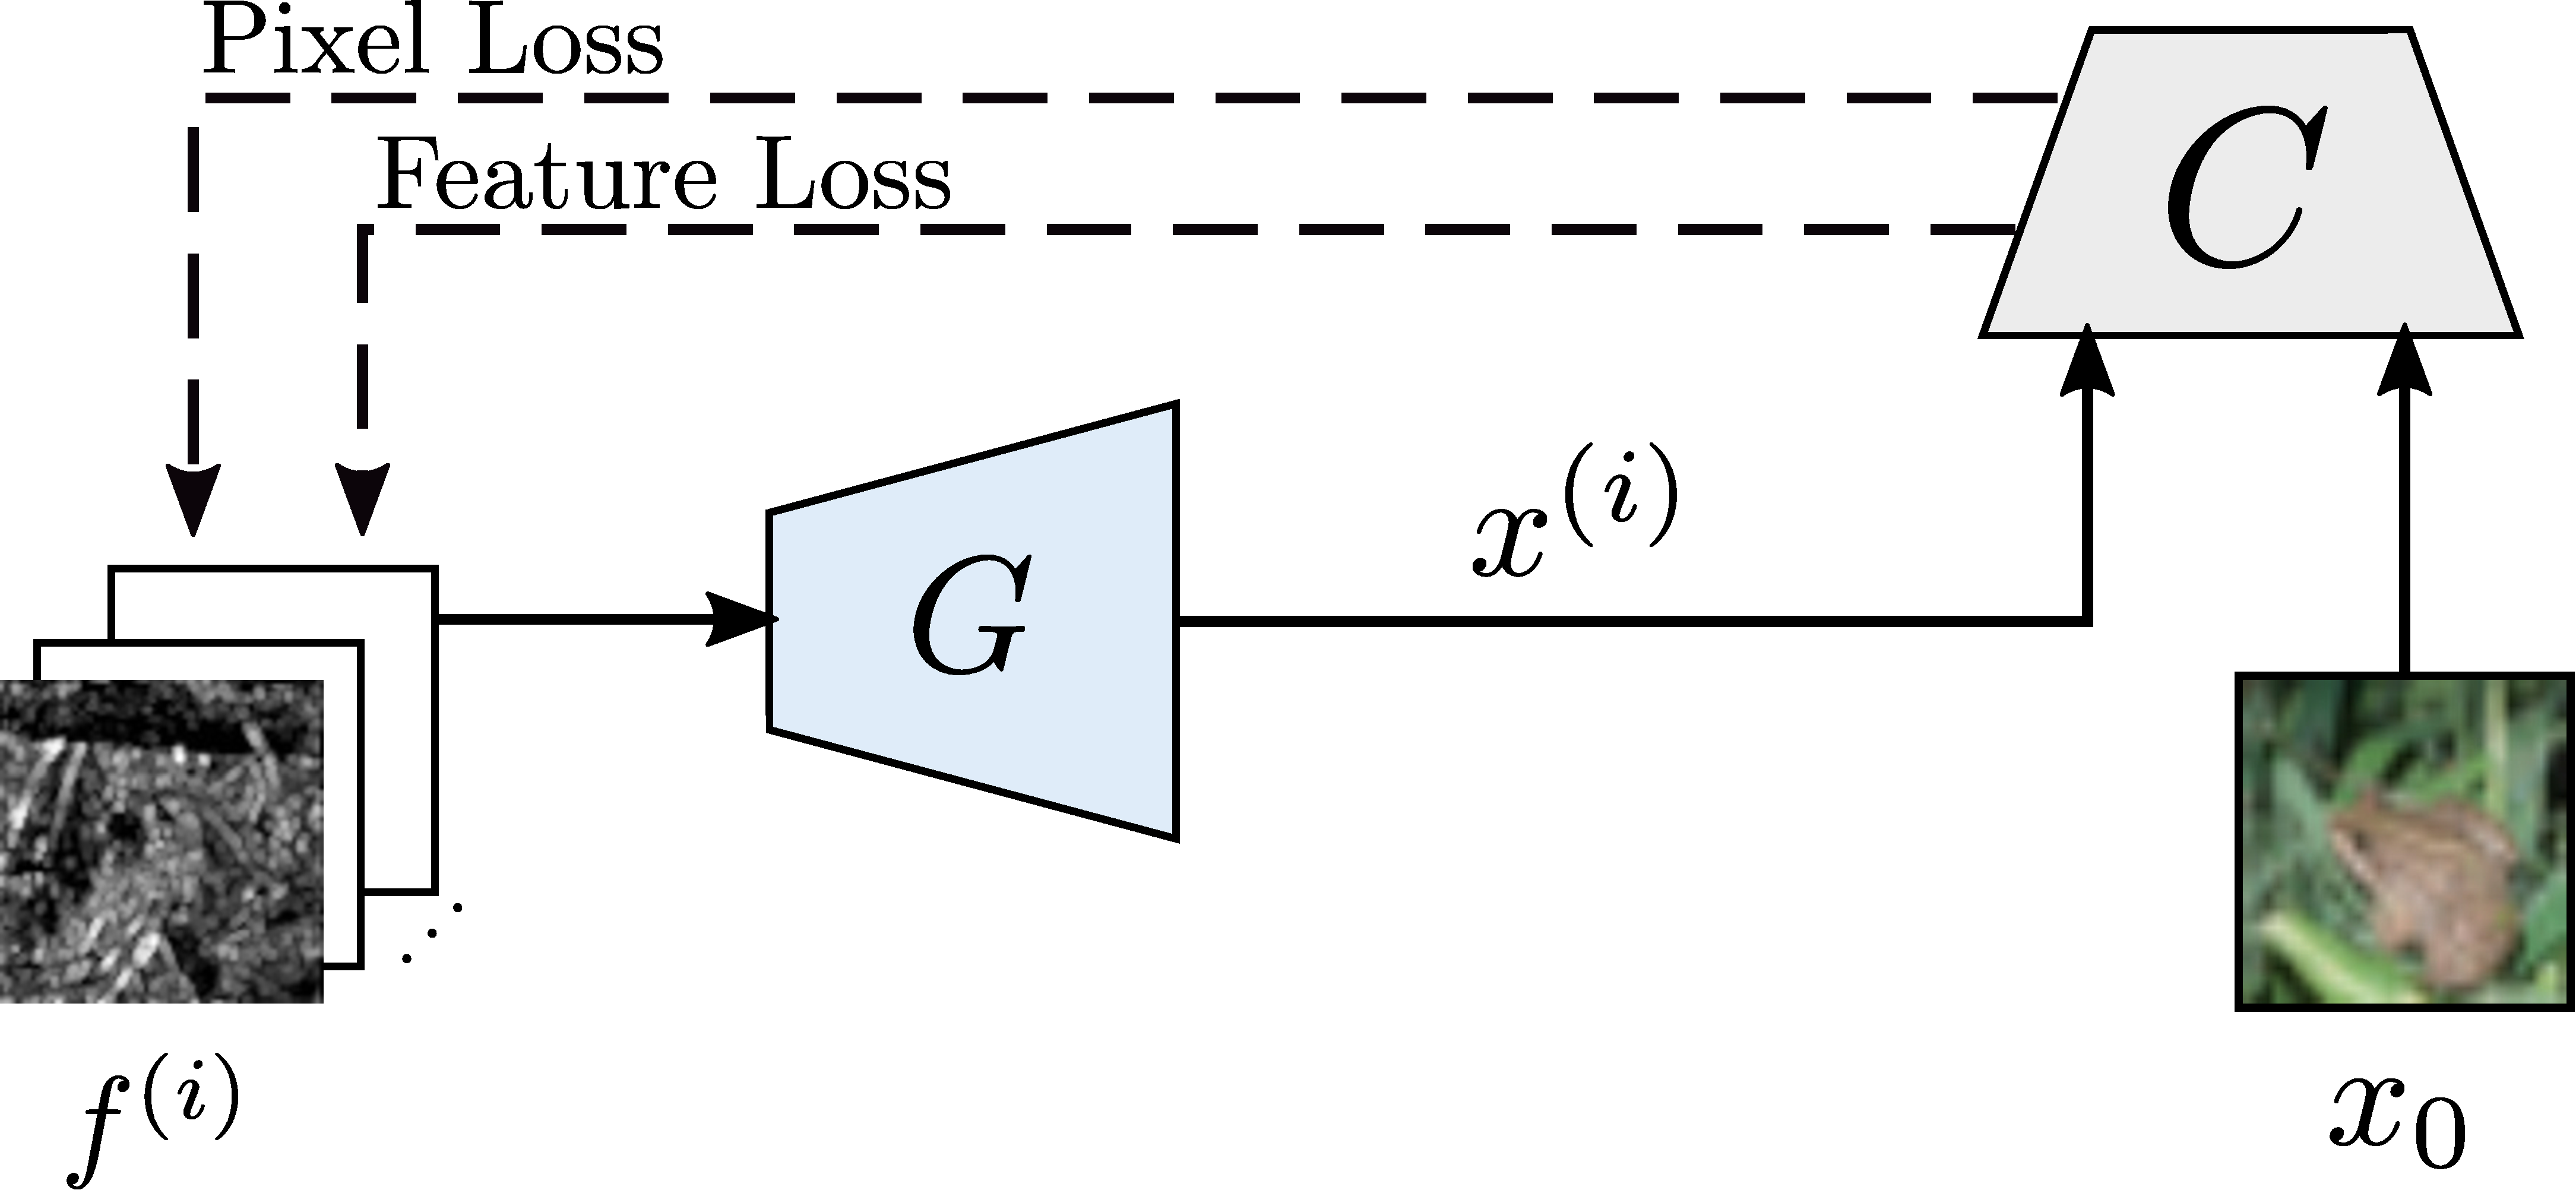
\includegraphics[width=0.475\textwidth]{figs/proposed/anomaly_diag.pdf}}\hspace{0.05\textwidth}
\subfloat[\textit{One-vs-All} Anomaly Detection]{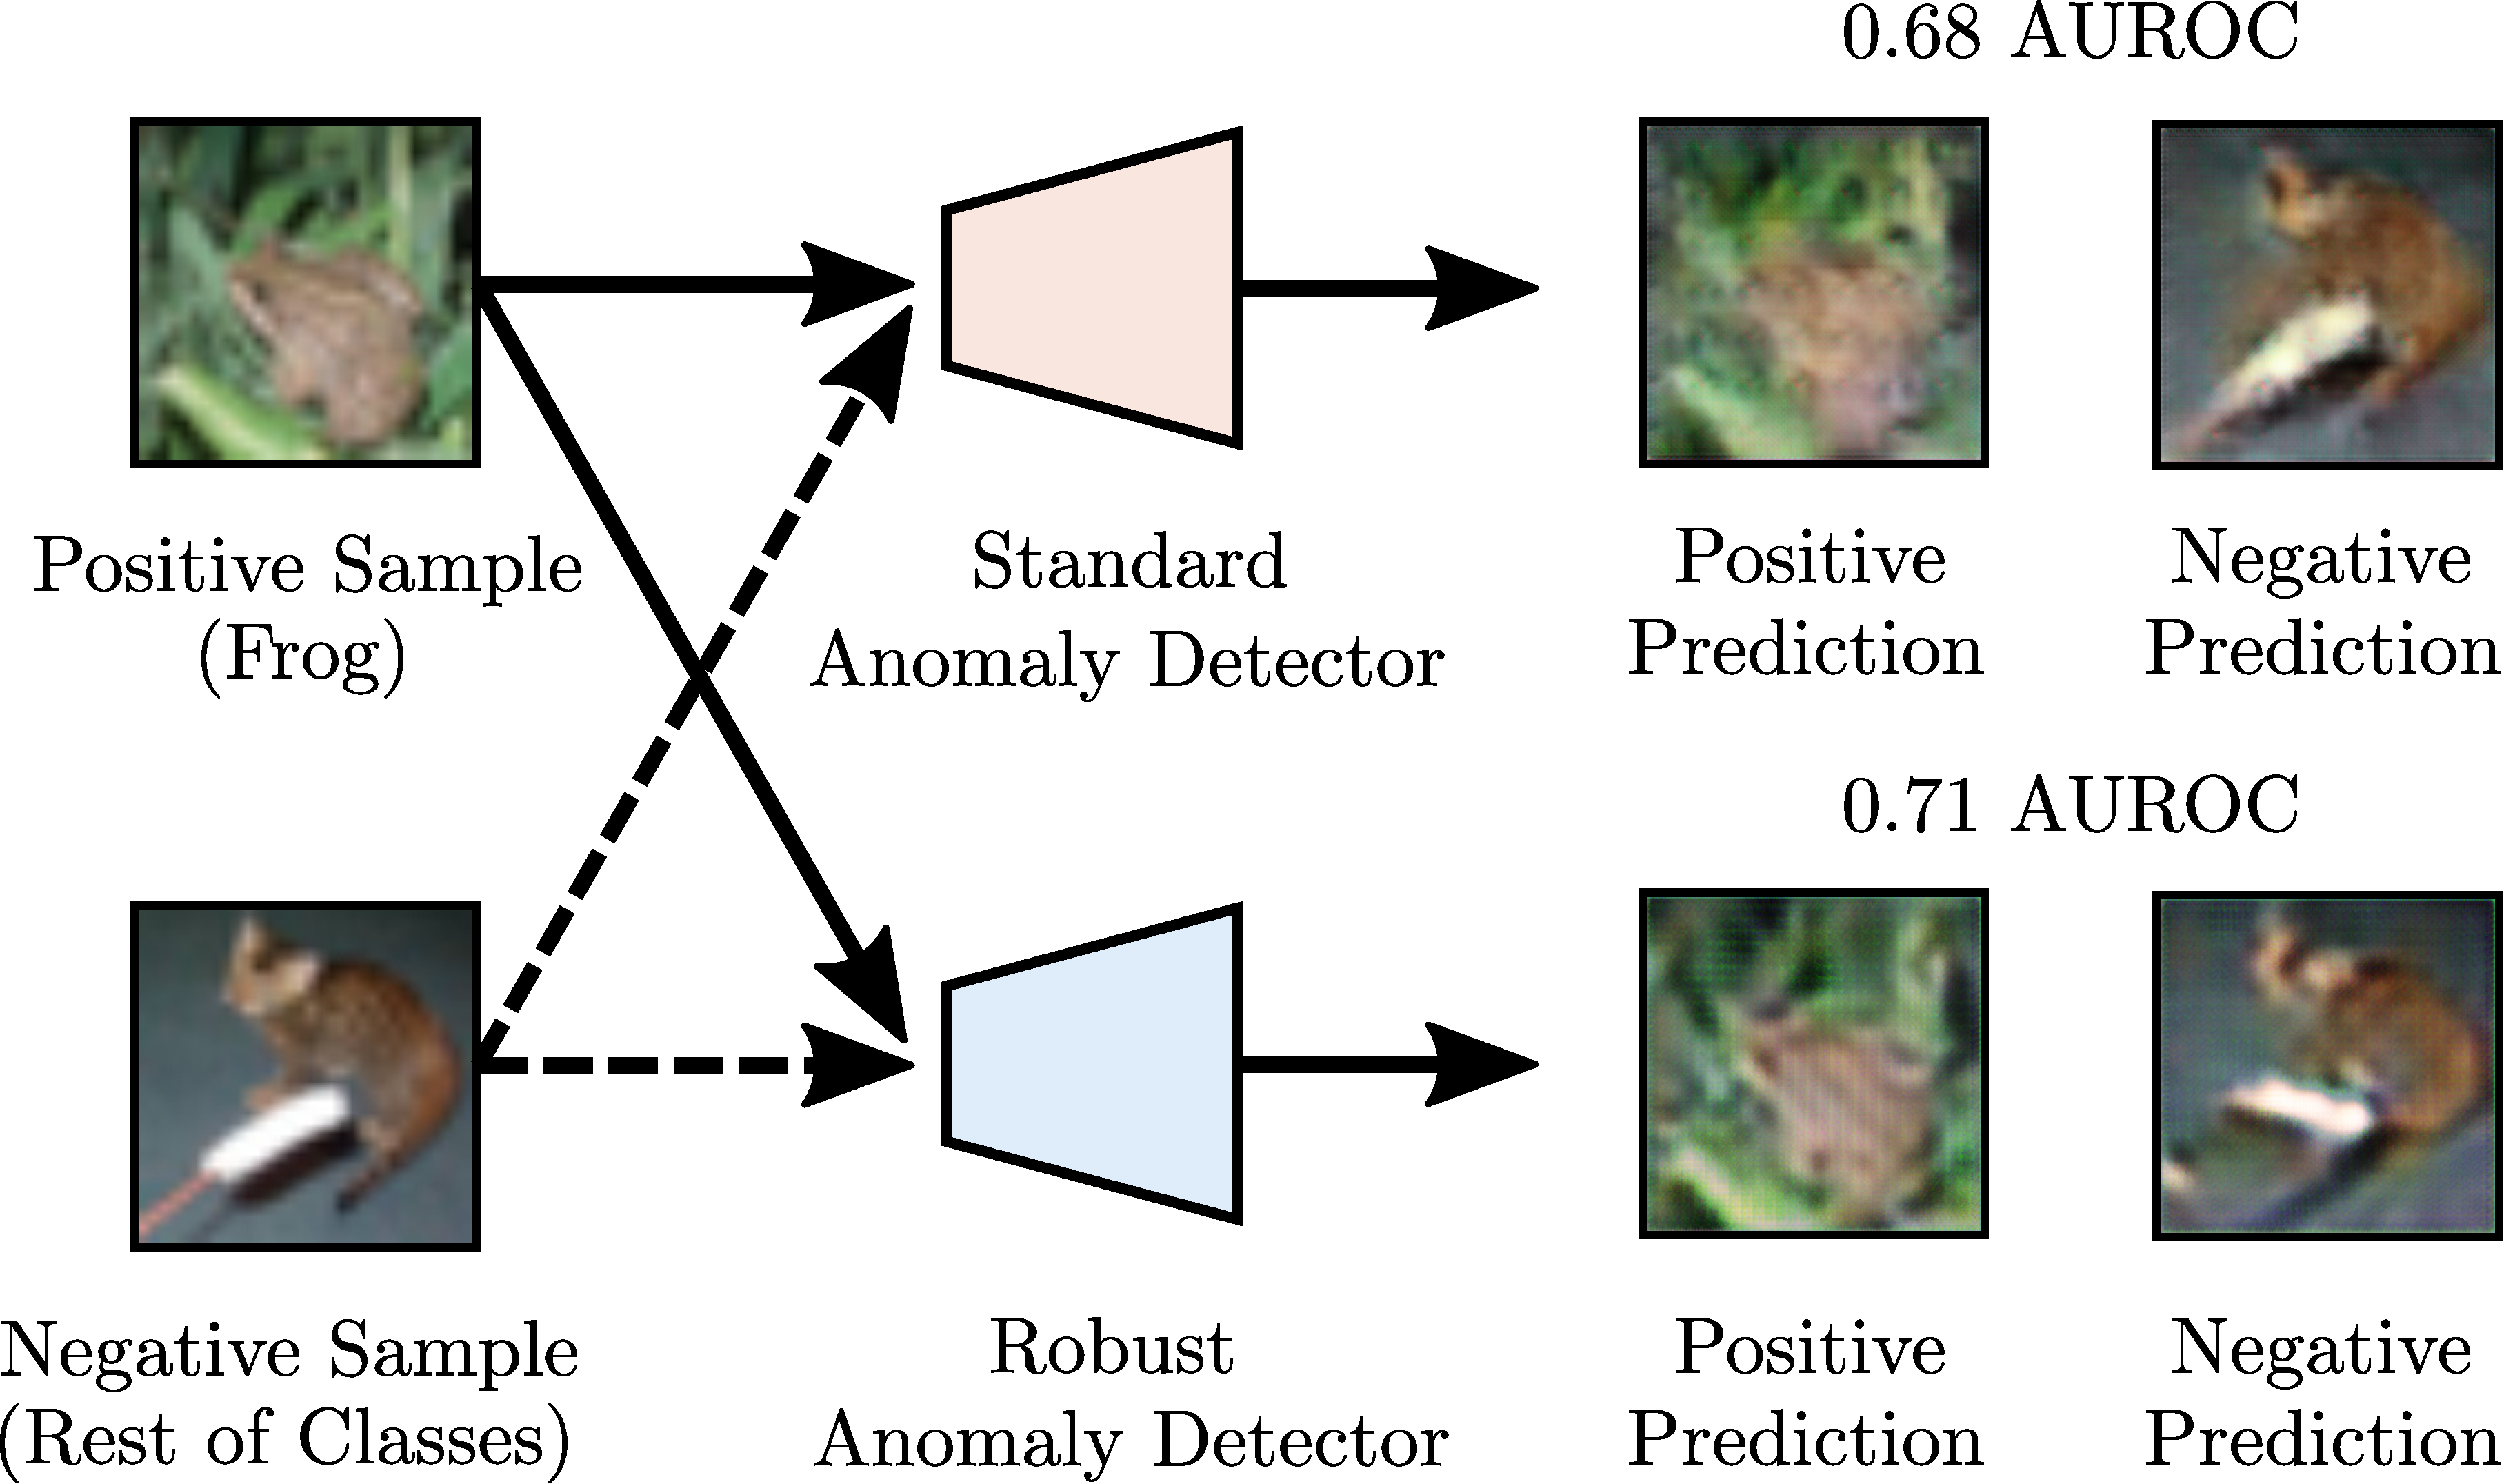
\includegraphics[width=0.405\textwidth]{figs/proposed/anomaly.pdf}}
\vspace{-0.2cm}
\caption{\label{fig:proposed_anomaly}Anomaly Detection using adversarially robust features.}
\vspace{-0.4 cm}
\end{figure}


\textbf{Experimental Setup.} We compare our technique using AR and standard features against ADGAN \cite{deecke_2018_image,golan_2018_deep}. We evaluate the performance on CIFAR10 and Cats vs. Dogs \cite{parkhi_2012_cats} datasets, where AUROC is computed on their full test sets.

Standard and AR encoders are fully-trained on ImageNet using the parameters described in \secref{sec:supp_results}. By freezing the encoder, generators are trained using pixel and feature losses on positives from the dataset of interest, CIFAR10 or Cats vs. Dogs. Input images are rescaled to $224 \times 224$ px. before being passed to the model, no additional data augmentation is applied during the generator training. The regularization parameters for both standard and AR autoencoders are heuristically selected as:
\vspace{-0.1\baselineskip}
\begin{itemize}
    \setlength\itemsep{0.1\baselineskip}
    \item Standard autoencoder: $\lambda_{\text{pix}}=2\times 10^{-3},\; \lambda_{\text{feat}}=1\times 10^{-2}$.
    \item AR autoencoder: $\lambda_{\text{pix}}=2\times 10^{-6},\; \lambda_{\text{feat}}=1\times 10^{-2}$.
\end{itemize}

\textbf{Iterative Optimization Details.} After training the generator on a particular class of interest, the optimal latent code $\hat{f}$ associated to an arbitrary target image $x$ is obtained via stochastic gradient descent. For both standard and AR autoencoders, the optimization criteria are identical to that used during the generator training. Specifically, we minimize pixel and feature loss components using the following hyperparameters:
\vspace{-0.1\baselineskip}
\begin{itemize}
    \setlength\itemsep{0.1\baselineskip}
    \item Standard autoencoder: $\alpha_{\text{pix}}=2\times 10^{-3},\; \alpha_{\text{feat}}=1\times 10^{-2}$.
    \item AR autoencoder: $\alpha_{\text{pix}}=2\times 10^{-6},\; \alpha_{\text{feat}}=1\times 10^{-2}$.
\end{itemize}

Detection is performed by solving Eq. \eqref{eq:anomaly_detection}, where $f\in \mathbb{R}^{6 \times 6 \times 256}$ is initialized as white Gaussian noise and optimized for $i_{\text{max}}=100$ iterations. The initial learn rate is chosen as $0.1$ and linearly decreases along iterations down to $0.001$.

\textbf{Results.} Full \textit{one-vs-all} anomaly detection results for CIFAR-10 and Cats vs. Dogs datasets are shown in \tabref{tab:supp_anomaly_detection}. On average, our AR model improves on outlier detection over its standard version and ADGAN. Our AR model gets $6.51\%$ and $8.84\%$ relative AUROC improvement over ADGAN on CIFAR-10 and Cats vs. Dogs, respectively. This shows our generator better distinguishes positives and negatives due to its improved reconstruction accuracy.
\begin{table}[t]
\small
\begin{center}
\resizebox{0.65\textwidth}{!}{
\begin{tabular}{c|c|c|c|c} 
\specialrule{.15em}{.05em}{.05em} 
Dataset & \makecell{Positive\\Class} & \makecell{ADGAN\\ \cite{deecke_2018_image}} & \makecell{Proposed\\(Standard)} & \makecell{Proposed\\(AR)}\\
\hline
\multirow{11}{*}{CIFAR-10} & $0$ & $0.649$ & $0.6874$ & $0.6533$\\
                        & $1$ & $0.39$ & $0.3498$ & $0.3755$\\
                        & $2$ & $0.652$ & $0.6756$ & $0.662$\\
                        & $3$ & $0.481$ & $0.5708$ & $0.6123$\\
                        & $4$ & $0.735$ & $0.751$ & $0.7538$\\
                        & $5$ & $0.476$ & $0.5101$ & $0.5278$\\
                        & $6$ & $0.623$ & $0.6895$ & $0.7113$\\
                        & $7$ & $0.487$ & $0.4773$ & $0.4526$\\
                        & $8$ & $0.66$ & $0.7232$ & $0.7008$\\
                        & $9$ & $0.378$ & $0.362$ & $0.4408$\\
\cline{2-5}
                        & Average & $0.553$ & $0.5797$ & $\mathbf{0.589}$\\
\hline
\multirow{3}{*}{\makecell{Cats vs. Dogs}}  & $0$ & $0.507$ & $0.663$ & $0.649$\\
                                            & $1$ & $0.481$ & $0.392$ & $0.427$\\
\cline{2-5}
                                            & Average & $0.494$ & $0.527$ & $\mathbf{0.538}$\\
\specialrule{.15em}{.05em}{.05em} 
\end{tabular}}
\end{center}
\vspace{-0.1 cm}
\caption{\label{tab:supp_anomaly_detection} AUROC of our proposed \textit{one-versus-all} anomaly detection method for each class. Detection evaluated on CIFAR-10 and Cats vs. Dogs datasets. Best results highlighted in black.}
\vspace{-0.5 cm}
\end{table}


\section{Additional Experiments on Feature Inversion}
\label{sec:supp_results}

\subsection{Ablation Study}
\label{sec:supp_results_ablation}

Feature inversion results obtained using different optimization criteria are illustrated in \figref{fig:supp_ablation}. Results clearly show the effect of each term, $\ell_{1}$ pixel, feature and GAN components, in the final reconstruction. Samples correspond to the ImageNet validation set. Particularly, when inverting features using pixel and feature losses, adversarially robust features show a significant improvement with respect to their standard counterparts. This agrees with the idea of adversarially robust features being perceptually aligned.
\begin{figure*}[t]
\subfloat[Ground-truth images.]{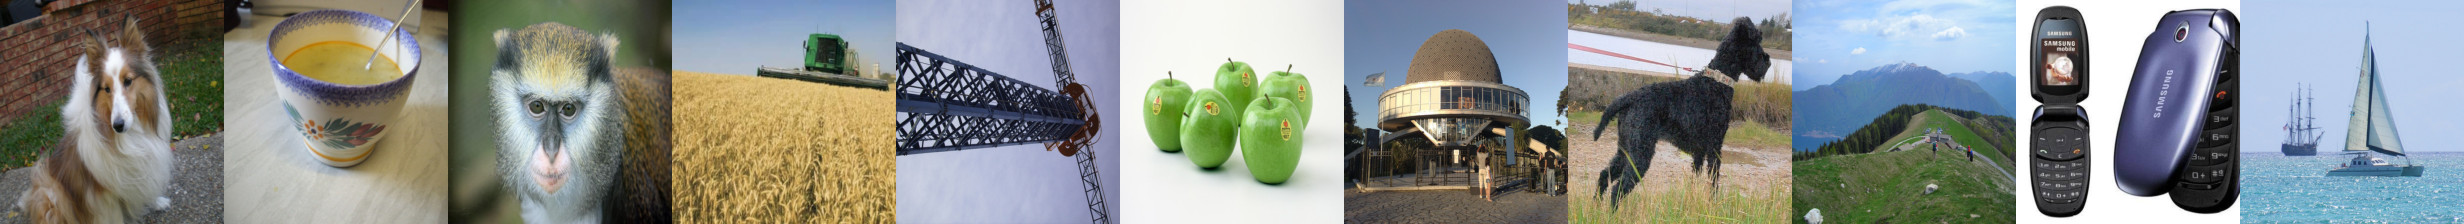
\includegraphics[width=\textwidth]{figs/ablation/ablation_00_gtruth.jpg}}

\vspace{-0.9\baselineskip}
\subfloat[Inverting standard (top) and AR (bottom) features using pixel losses.]{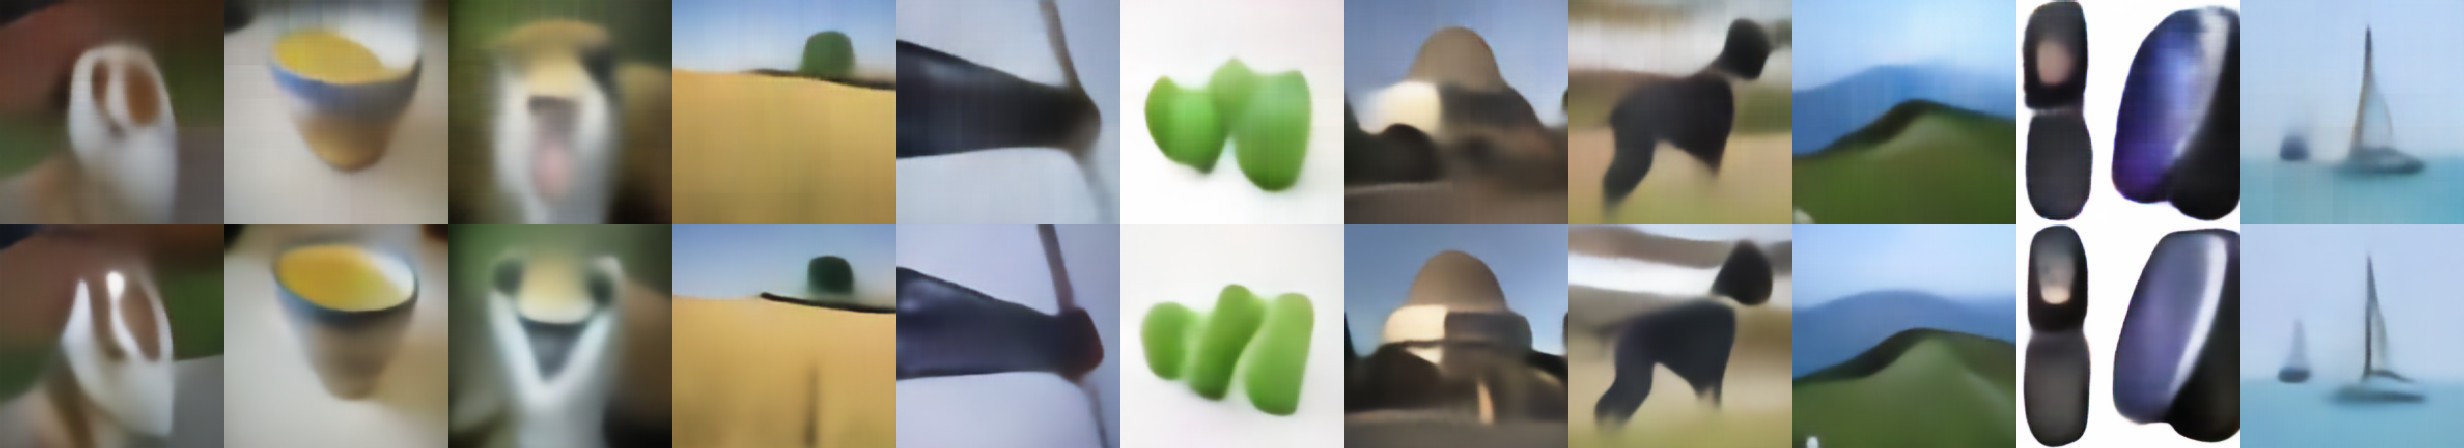
\includegraphics[width=\textwidth]{figs/ablation/ablation_01_pix.jpg}}

\vspace{-0.9\baselineskip}
\subfloat[Inverting standard (top) and AR (bottom) features using pixel and feature losses.]{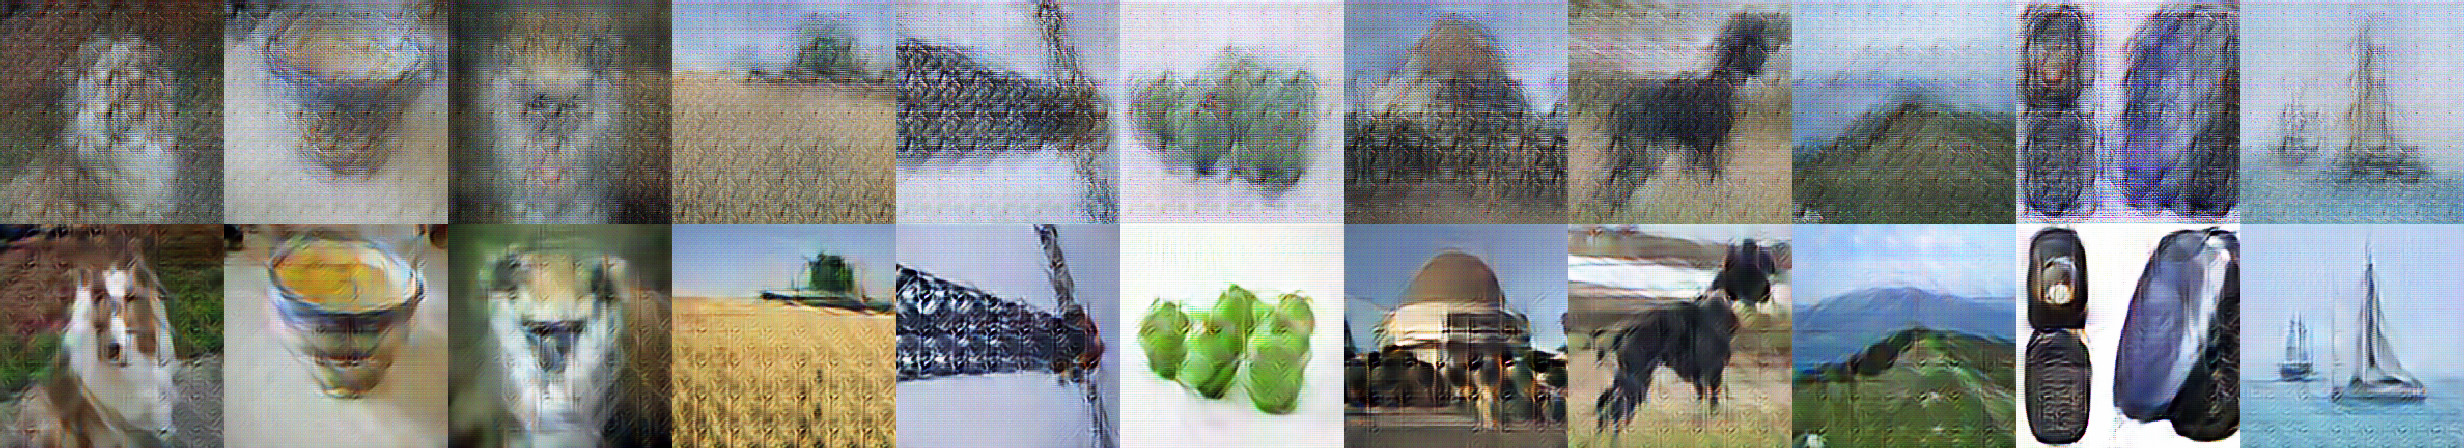
\includegraphics[width=\textwidth]{figs/ablation/ablation_02_pix_feat.jpg}}

\vspace{-0.9\baselineskip}
\subfloat[Inverting standard (top) and AR (bottom) features using pixel, feature and GAN losses.]{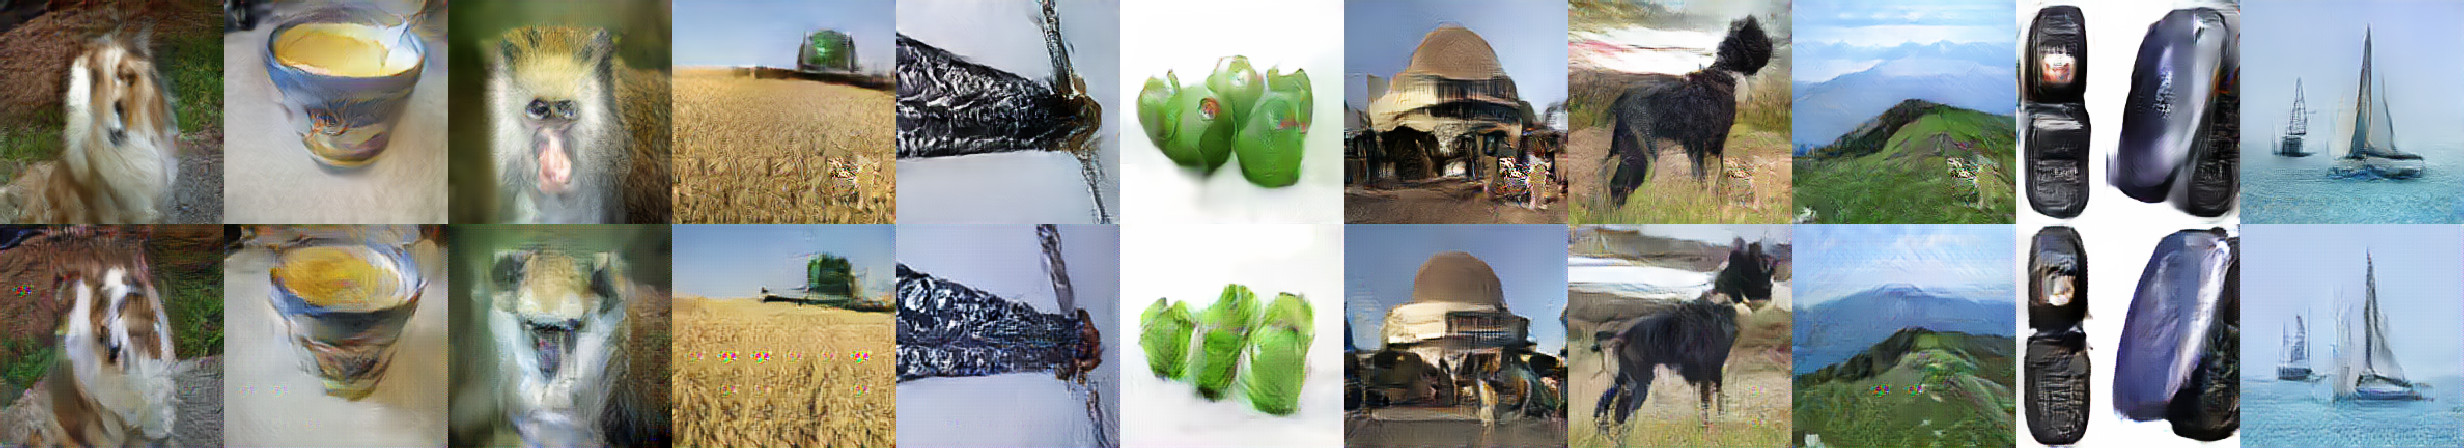
\includegraphics[width=\textwidth]{figs/ablation/ablation_03_pix_feat_gan.jpg}}

\caption{CNN-based feature inversion of standard and AR representations. AlexNet \layer{Conv5} \textbf{standard (top)} and \textbf{AR (bottom)} features are inverted using an image generator trained on (a) $\ell_{1}$ Pixel loss, (b) Pixel and feature losses, and (c) Pixel, feature and GAN losses.}
\label{fig:supp_ablation}
\end{figure*}


\subsection{Robustness to Scale Changes}
\label{sec:supp_results_scale}
Inversion accuracy on upscaled low-resolution images is illustrated in \figref{fig:sup_hires01} for scale factors $L\in \{1,\dots, 10\}$. While standard inversions show significant distortions for large upscaling factors $L$, reconstructions from adversarially robust representations show almost perfect reconstruction for high upscaling factors. Quantitative results are included in \tabref{tab:supp_hires01}. Results improve almost monotonically when inverting AR representations, even without exposing the Autoencoder to high-resolution images during training and without any fine-tuning.

On the other hand, extended results on feature inversion from high-resolution images are illustrated in \figref{fig:supp_hires02}. Notice that, in contrast to the previous case, input samples correspond to natural high-resolution images and are encoded without any scaling. Results show a good color and edge preservation from our AR autoencoder, while inverting standard features show bogus components and noticeable color distortions.
\begin{figure*}[t]
\centering
\begin{minipage}{0.09\textwidth}
\centering\textbf{\hspace{-0.5\baselineskip}\scalebox{0.7}{G. truth}}
\end{minipage}\begin{minipage}{0.09\textwidth}
\centering \scalebox{0.7}{$L= 1$}
\end{minipage}\begin{minipage}{0.09\textwidth}
\centering \scalebox{0.7}{$L= 2$}
\end{minipage}\begin{minipage}{0.09\textwidth}
\centering \scalebox{0.7}{$L= 3$}
\end{minipage}\begin{minipage}{0.09\textwidth}
\centering \scalebox{0.7}{$L= 4$}
\end{minipage}\begin{minipage}{0.09\textwidth}
\centering \scalebox{0.7}{$L= 5$}
\end{minipage}\begin{minipage}{0.09\textwidth}
\centering \scalebox{0.7}{$L= 6$}
\end{minipage}\begin{minipage}{0.09\textwidth}
\centering \scalebox{0.7}{$L= 7$}
\end{minipage}\begin{minipage}{0.09\textwidth}
\centering \scalebox{0.7}{$L= 8$}
\end{minipage}\begin{minipage}{0.09\textwidth}
\centering \scalebox{0.7}{$L= 9$}
\end{minipage}\begin{minipage}{0.09\textwidth}
\centering \scalebox{0.7}{$L= 10$}
\end{minipage}\vspace{0.5\baselineskip}

\vspace{-0.5 cm}
\subfloat{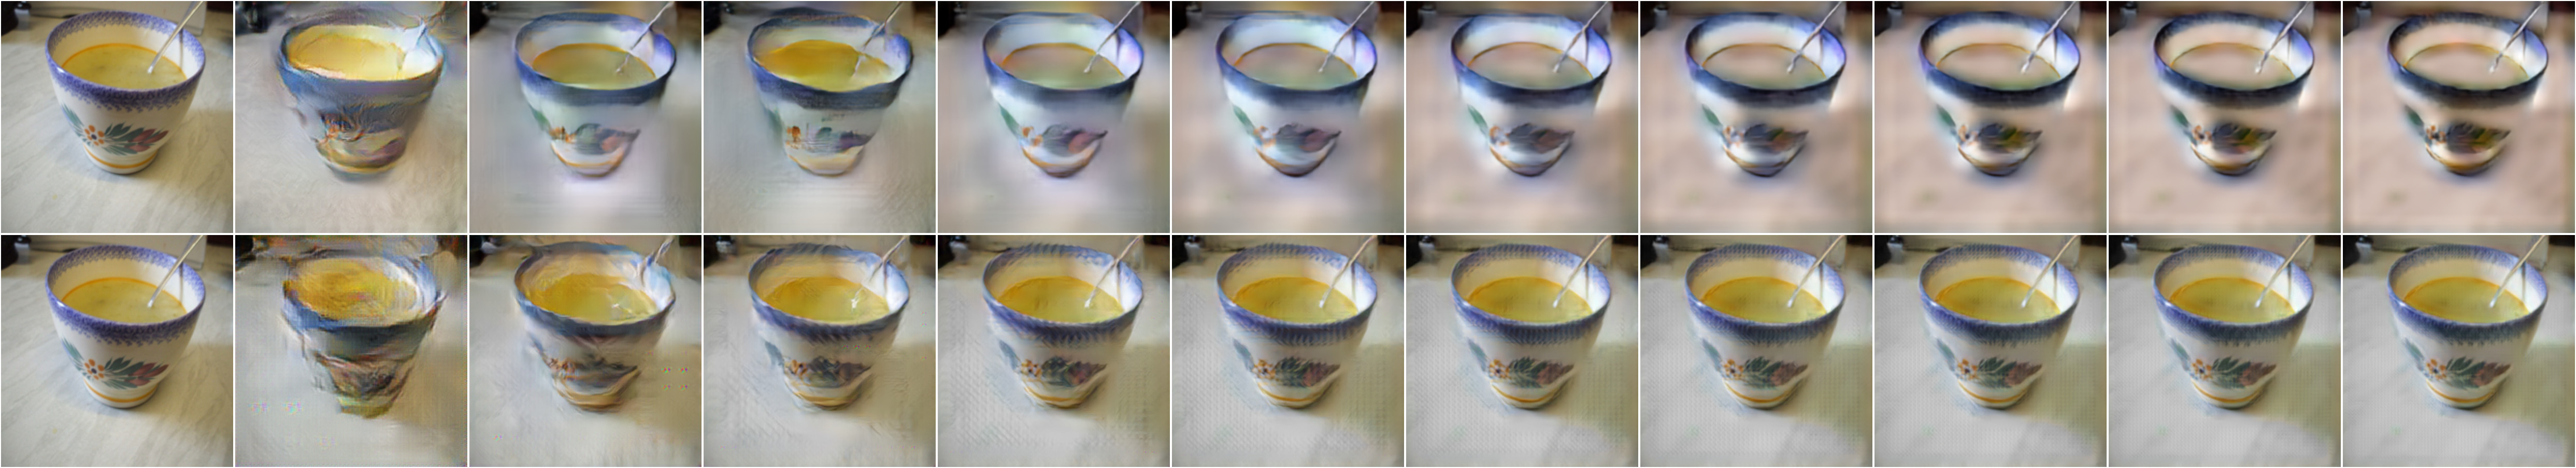
\includegraphics[width=1\textwidth]{figs/upscaling/tile_group_hires02_1.jpg}}

\vspace{-.9\baselineskip}
\subfloat{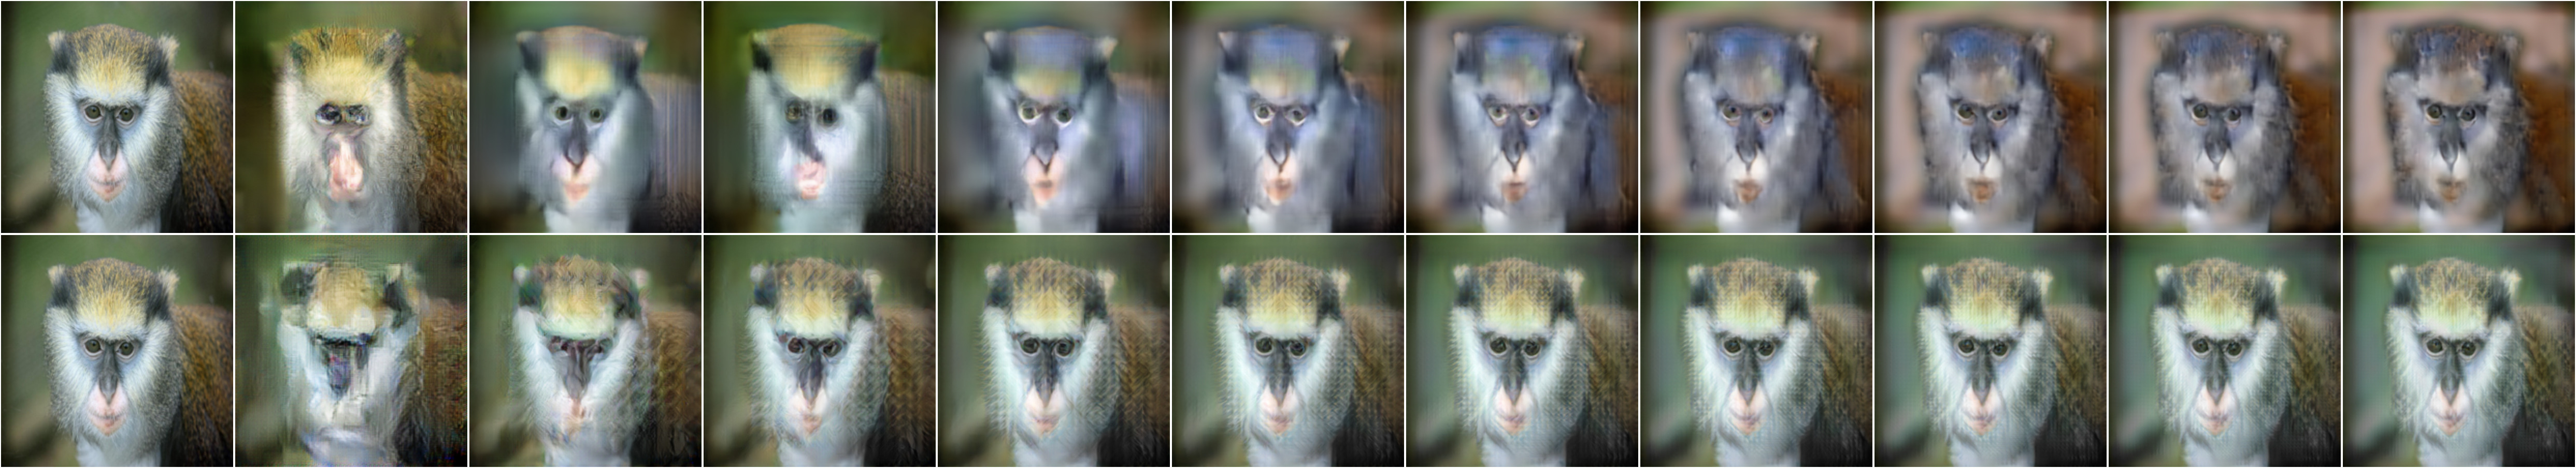
\includegraphics[width=1\textwidth]{figs/upscaling/tile_group_hires02_2.jpg}}

\vspace{-.9\baselineskip}
\subfloat{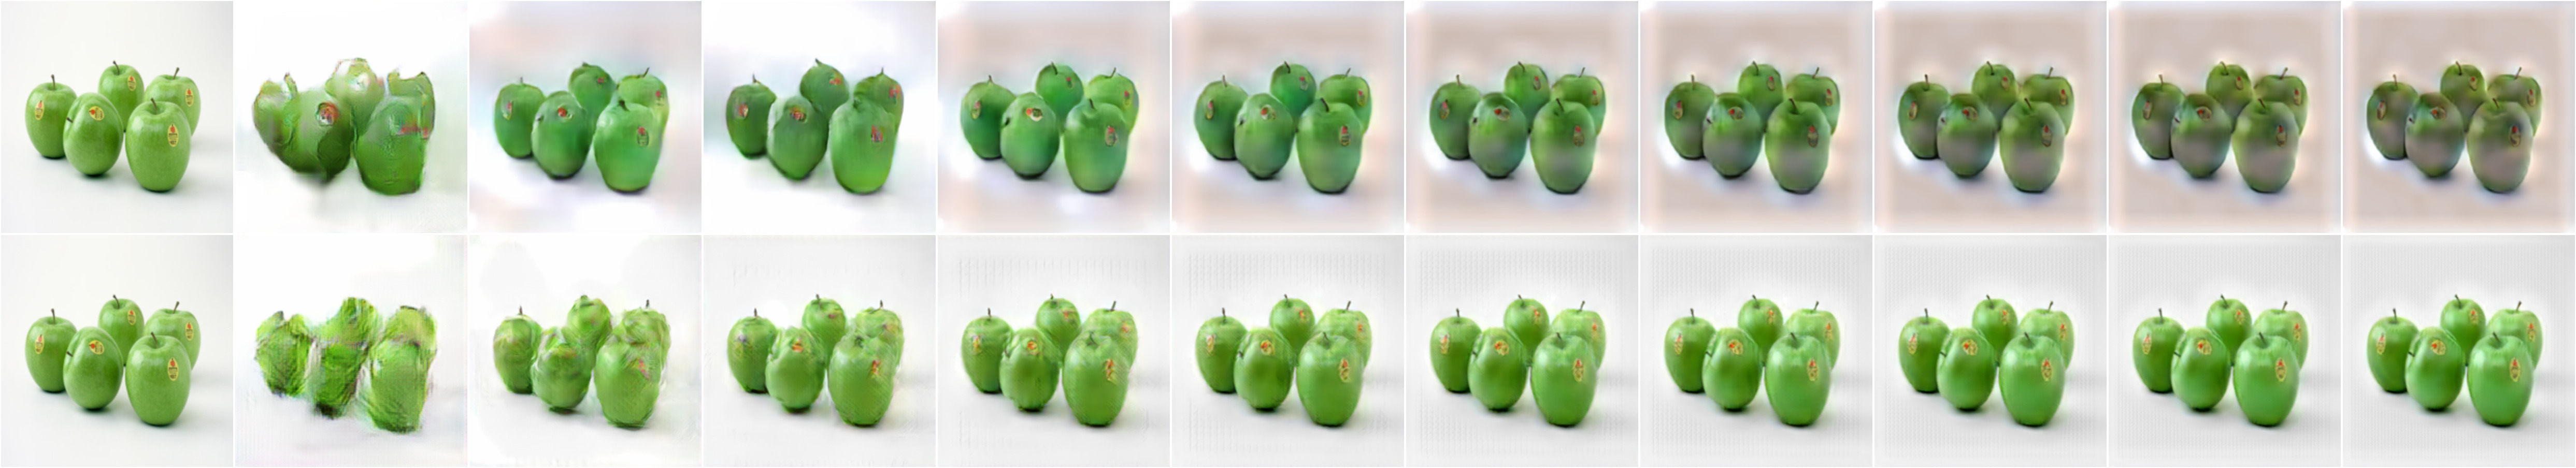
\includegraphics[width=1\textwidth]{figs/upscaling/tile_group_hires02_5.jpg}}

\vspace{-.9\baselineskip}
\subfloat{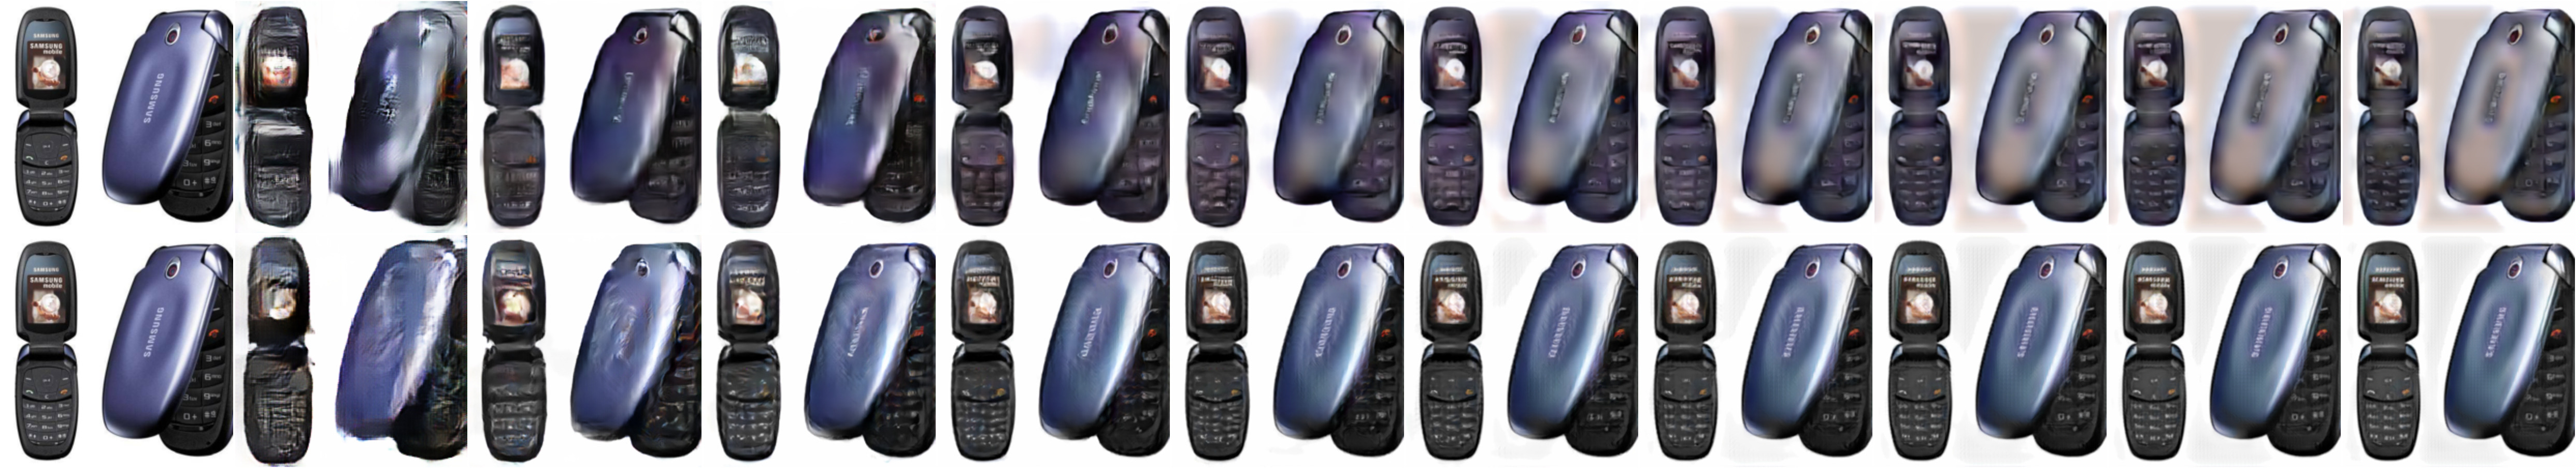
\includegraphics[width=1\textwidth]{figs/upscaling/tile_group_hires02_9.jpg}}

\caption{Reconstructing upscaled images. Upscaled ImageNet samples are inverted from their standard and AR representations. While standard representations (top row) are severely degraded, AR representations (bottom row) show an outstanding accuracy that improves with the scaling factor.}
\label{fig:sup_hires01}
\end{figure*}

\begin{table*}[t]
\small
\centering
\begin{center}
\resizebox{0.9\textwidth}{!}{
\def\arraystretch{1.25}
\begin{tabular}{c|c|c|c|c|c|c}
\specialrule{.15em}{.05em}{.05em} 
\multirow{2}{*}{\makecell{$L$}} & \multicolumn{3}{c|}{Standard AlexNet} & \multicolumn{3}{c}{Robust AlexNet} \\
\cline{2-7}
& PSNR (dB)$\uparrow$ & SSIM$\uparrow$ & LPIPS$\downarrow$ & PSNR (dB)$\uparrow$ & SSIM$\uparrow$ & LPIPS$\downarrow$\\
\hline
 $1\ (224 \times 224)$ & \makecell{$15.057$} & \makecell{$0.3067$} & \makecell{$0.5473$} & \makecell{$17.2273$} & \makecell{$0.3580$} & \makecell{$0.5665$}\\
 $2\ (448 \times 448)$ & $16.2777$ & $0.4068$ & $0.4234$ & $20.3554$ & $0.4859$ & $0.469$\\
 $3\ (672 \times 672)$ & $16.0668$ & $0.4317$ & $0.4143$ & $21.3696$ & $0.5265$ & $0.4376$\\
 $4\ (896 \times 896)$ & \makecell{$15.4258$} & \makecell{$0.4655$} & \makecell{$0.4136$} & \makecell{$22.575$} & \makecell{$0.5892$} & \makecell{$0.4012$}\\
 $5\ (1120 \times 1120)$ & $14.9726$ & $0.4753$ & $0.4235$ & $22.9861$ & $0.6074$ & $0.4018$\\
 $6\ (1344 \times 1344)$ & $14.3093$ & $0.4887$ & $0.4358$ & $23.4824$ & $0.6527$ & $0.383$\\
 $7\ (1568 \times 1568)$ & \makecell{$13.8922$} & \makecell{$0.4852$} & \makecell{$0.4587$} & \makecell{$23.5778$} & \makecell{$0.6588$} & \makecell{$0.3898$}\\
 $8\ (1792 \times 1792)$ & $13.4781$ & $0.4967$ & $0.4656$ & $23.7604$ & $0.70178$ & $0.3638$\\
 $9\ (2016 \times 2016)$ & $13.2869$ & $0.4882$ & $0.4834$ & $23.7907$ & $0.6924$ & $0.3906$\\
 $10\ (2240 \times 2240)$ & \makecell{$13.1013$} & \makecell{$0.4969$} & \makecell{$0.486$} & \makecell{$23.9566$} & \makecell{$0.7244$} & \makecell{$0.3892$}\\
\specialrule{.15em}{.05em}{.05em} 
\end{tabular}}
\end{center}

\vspace{-0.3 cm}
\caption{\label{tab:supp_hires01} Reconstructing upscaled images ($L\in\{1,\dots,10\}$). Upscaled $224 \times 224$ ImageNet samples are reconstructed from standard and AR AlexNet features, the latter predominantly obtaining higher accuracy.}
\vspace{-0.6 cm}
\end{table*}

\begin{figure*}[t]
\begin{minipage}[t]{0.166\textwidth}
\centering\textbf{\scriptsize{Ground-truth}}
\end{minipage}\begin{minipage}[t]{0.166\textwidth}
\centering \textbf{\scriptsize{Standard}}
\end{minipage}\begin{minipage}[t]{0.166\textwidth}
\centering \textbf{\scriptsize{AR (ours)}}
\end{minipage}\begin{minipage}[t]{0.166\textwidth}
\centering\textbf{\scriptsize{Ground-truth}}
\end{minipage}\begin{minipage}[t]{0.166\textwidth}
\centering \textbf{\scriptsize{Standard}}
\end{minipage}\begin{minipage}[t]{0.166\textwidth}
\centering \textbf{\scriptsize{AR (ours)}}
\end{minipage}

\vspace{-0.8\baselineskip}
\subfloat[]{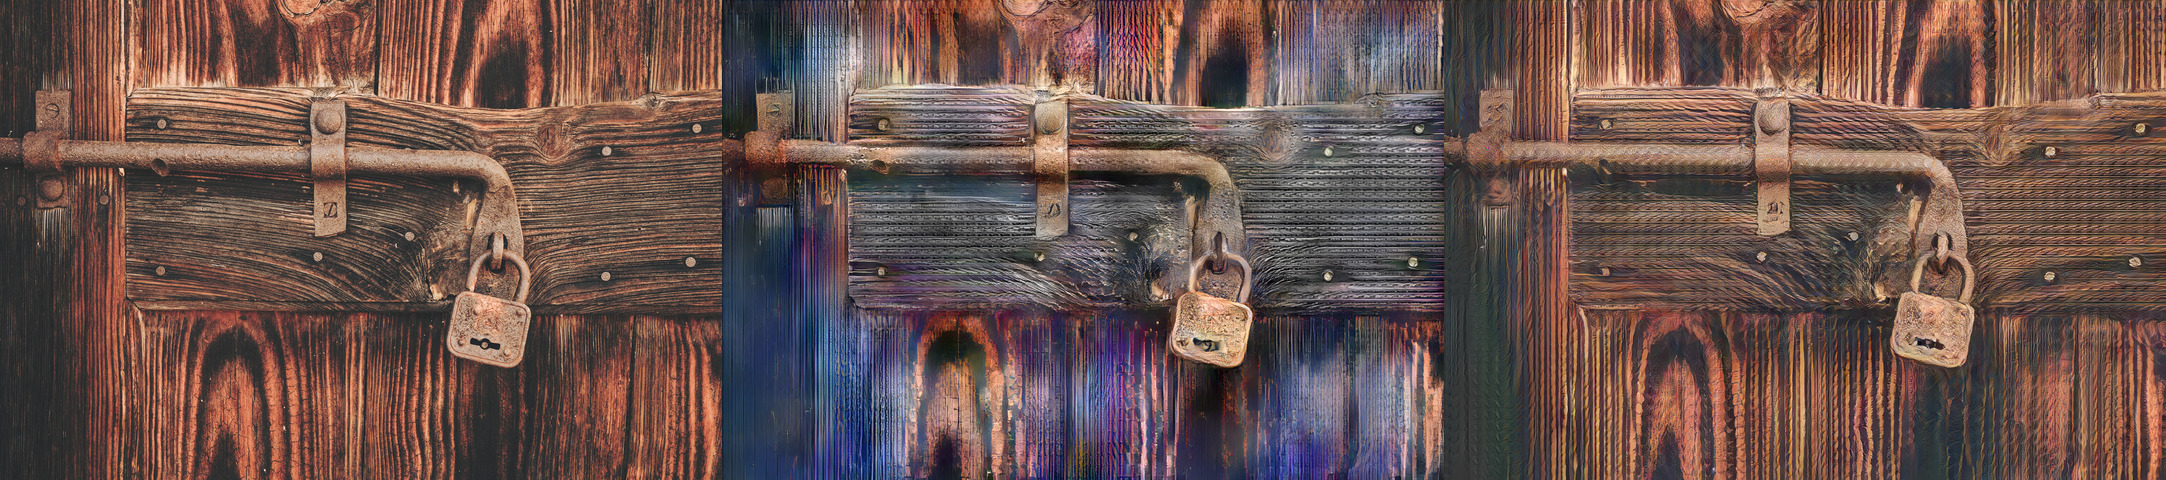
\includegraphics[width=0.5\textwidth]{figs/hires/tile_hires01_1.jpg}}
\subfloat[]{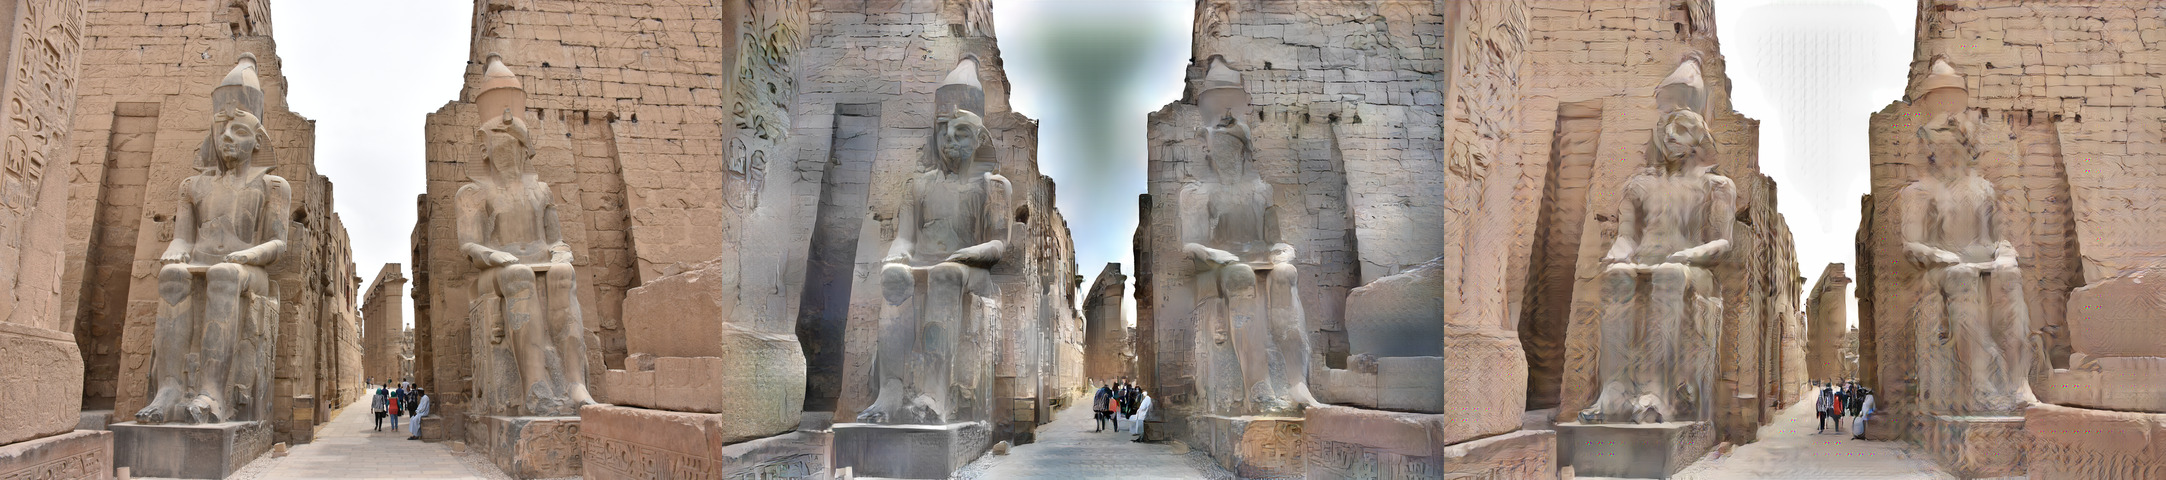
\includegraphics[width=0.5\textwidth]{figs/hires/tile_hires01_12.jpg}}

\vspace{-.9\baselineskip}
\subfloat[]{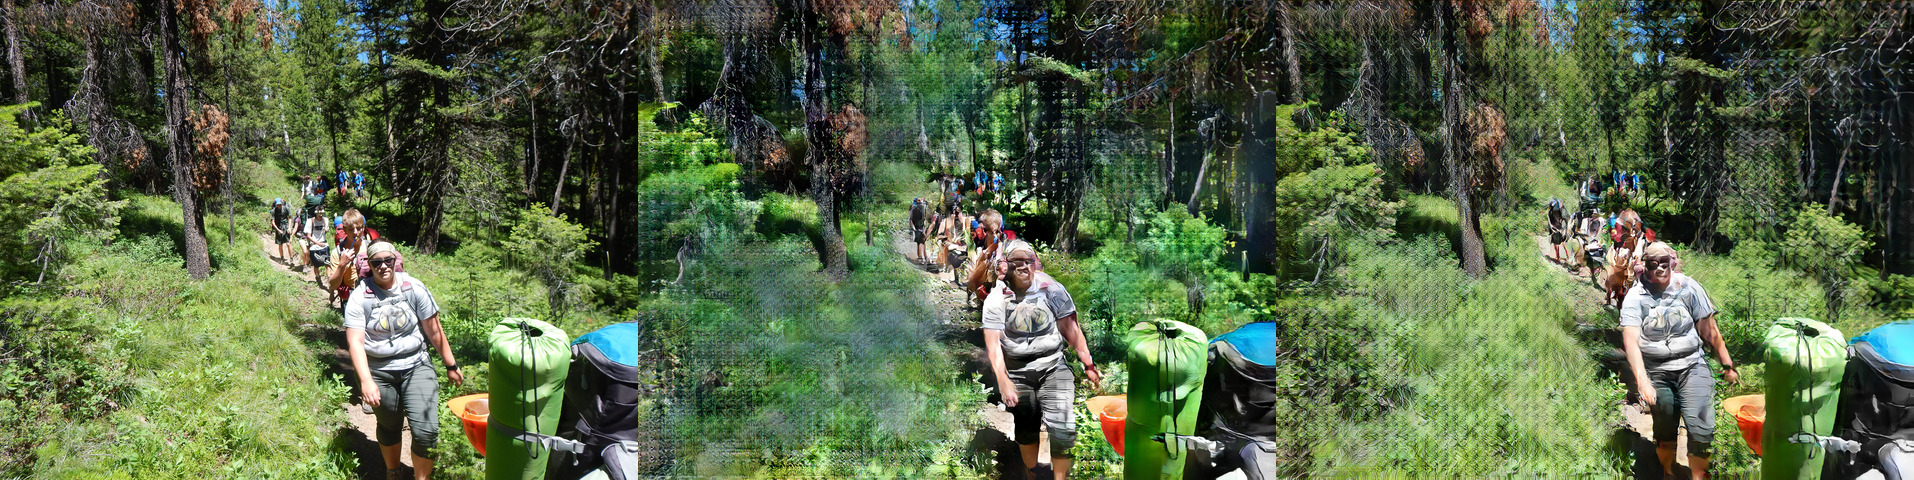
\includegraphics[width=0.472\textwidth]{figs/hires/tile_hires01_0.jpg}}
\subfloat[]{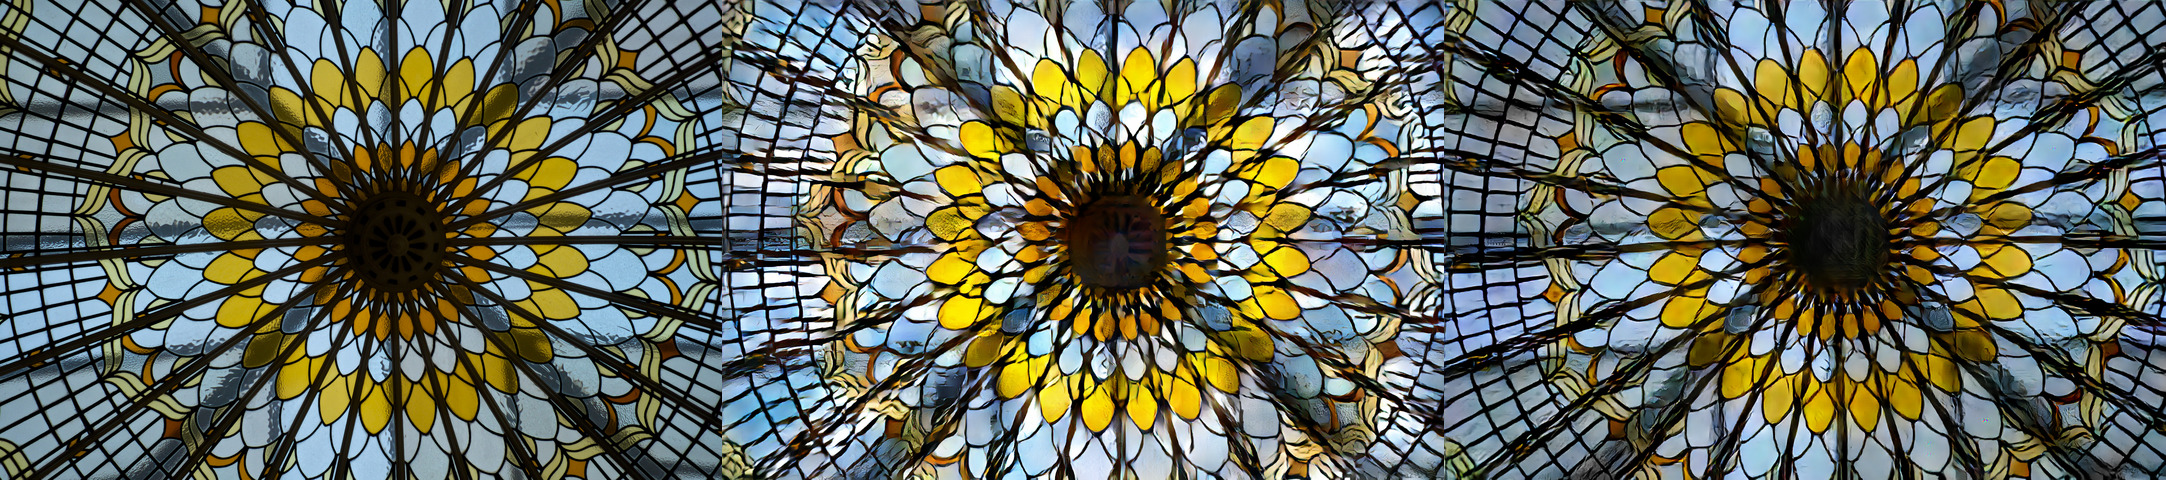
\includegraphics[width=0.528\textwidth]{figs/hires/tile_hires01_6.jpg}}

\vspace{-.9\baselineskip}
\subfloat[]{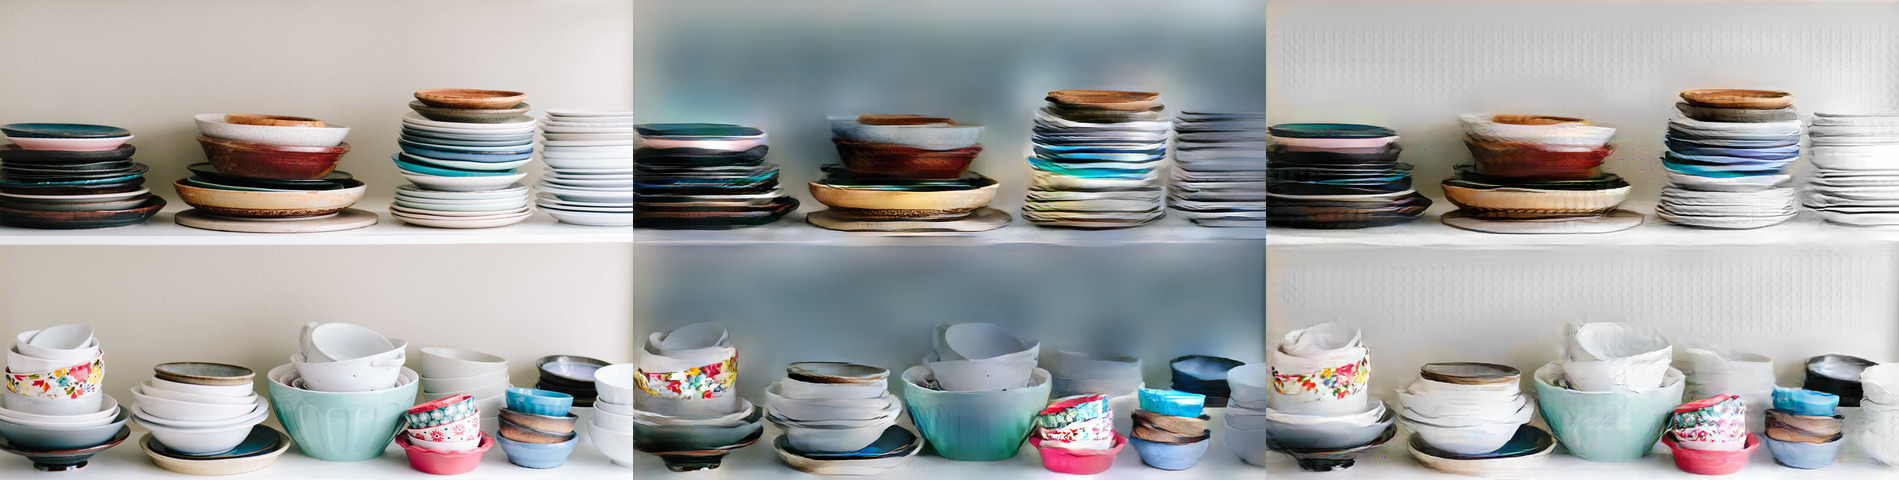
\includegraphics[width=0.45\textwidth]{figs/hires/tile_hires01_3.jpg}}
\subfloat[]{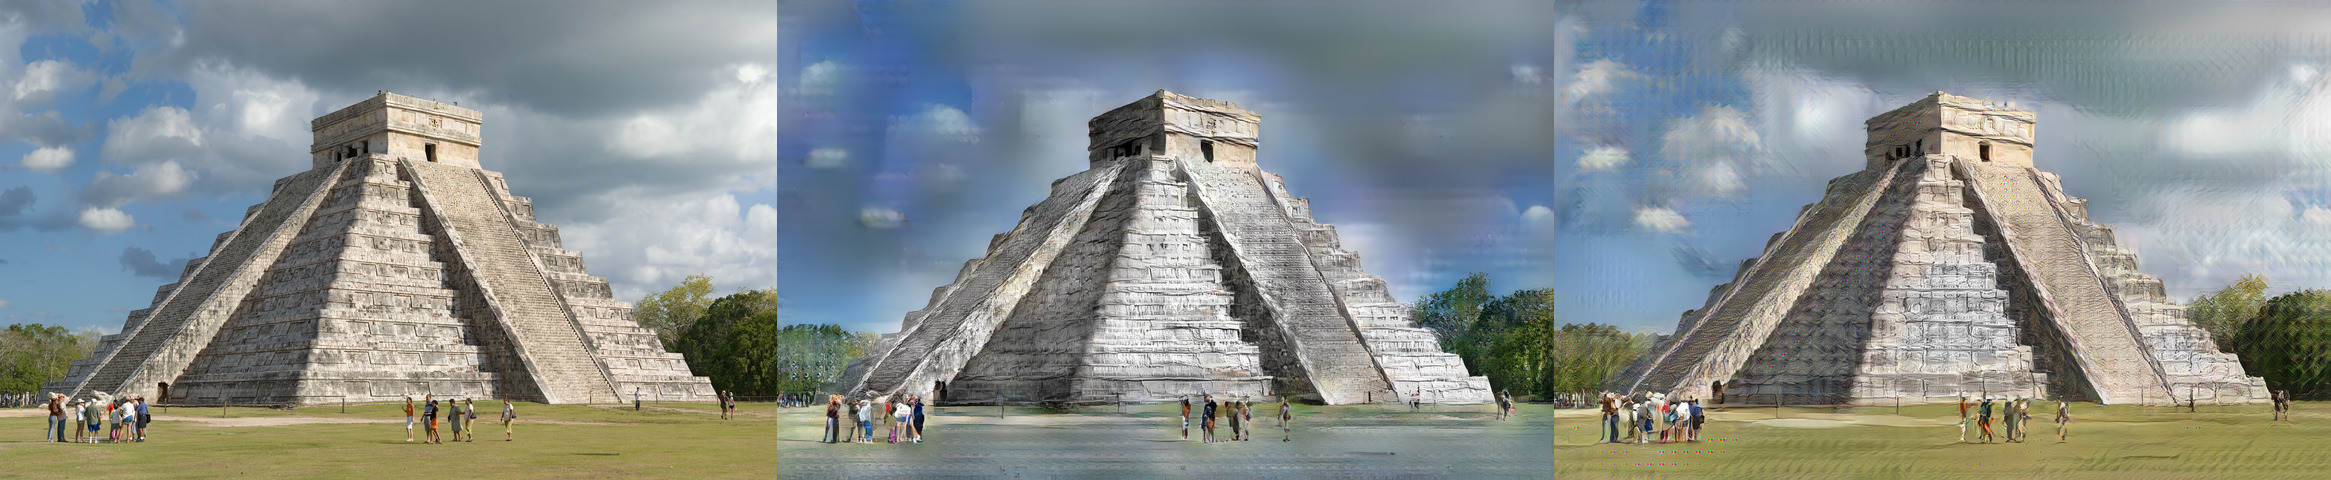
\includegraphics[width=0.55\textwidth]{figs/hires/tile_hires01_8.jpg}}

\vspace{-.9\baselineskip}
\subfloat[]{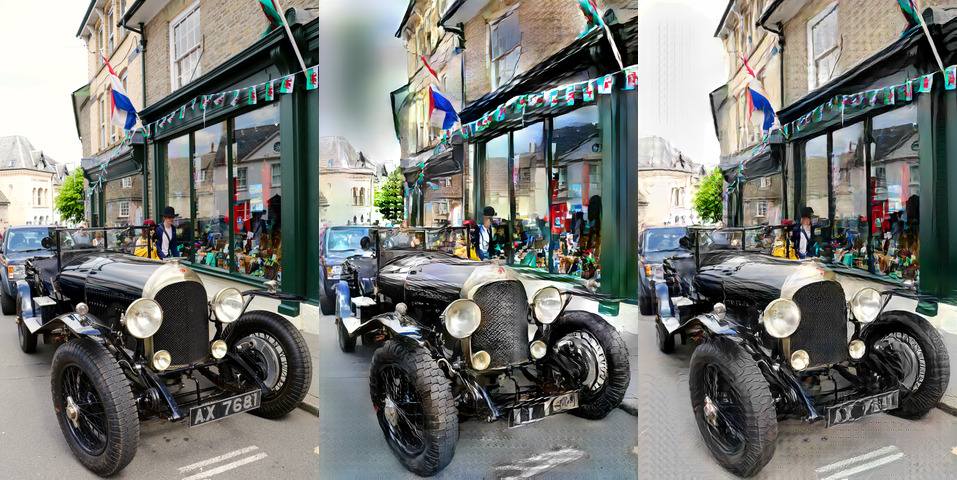
\includegraphics[width=0.5\textwidth]{figs/hires/tile_hires01_4.jpg}}
\subfloat[]{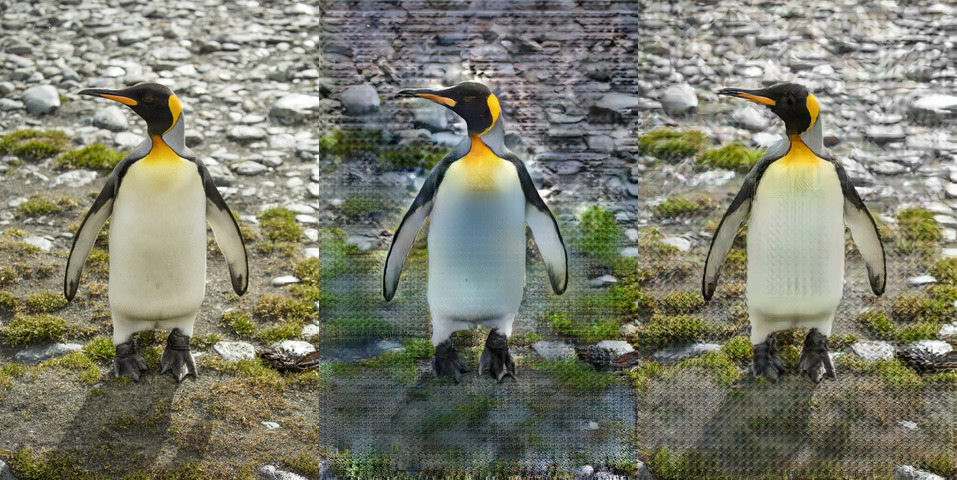
\includegraphics[width=0.5\textwidth]{figs/hires/tile_hires01_2.jpg}}

\vspace{-.3 cm}
\caption{At a resolution of $2040\times 1536$, $10$ times higher than the training resolution, standard reconstructions show color and structure degradation. In contrast, reconstructions from our AR autoencoder do not suffer from such distortions and are closer to target DIV2K images.}
\label{fig:supp_hires02}
\end{figure*}


\subsection{ResNet-18: Robustness Level vs. Reconstruction Accuracy}
\label{sec:supp_inverting_alternative}

We take the ResNet-18 model trained on CIFAR-10 from the \textit{Robustness} library \cite{robustness}, invert its third residual block ($4 \times 4 \times 512$) based on our approach using pixel and feature losses, and evaluate its reconstruction accuracy for standard and AR cases.

We measure the reconstruction accuracy for different robustness levels by training six AR classifiers via $\ell_{2}$ PGD attacks (Madry et al.) with attack radii $\varepsilon$ covering from $0$ to $3.5$ (see \tabref{tab:accuracy02_1}). Accuracy for each model is measured in terms of PSNR, SSIM and LPIPS. We also report the robustness obtained by each model against $\ell_{2}$ PGD attacks.
\begin{table*}[b]
\small
\begin{center}
\resizebox{0.9\textwidth}{!}{
\begin{tabular}{c|c|c|c|c|c|c|c|c} 
\specialrule{.15em}{.05em}{.05em}
&\multicolumn{8}{c}{$\ell_{2}$ PGD Attack ($\varepsilon$)}\\
\cline{2-9}
& $0$ & $0.5$ & $1$ & $1.5$ & $2$ & $2.5$ & $3$ & $3.5$ \\
\hline
\makecell{Standard Accuracy} & $94.93$ & $88.28$ & $81.07$ & $72.47$ & $64.48$ & $64.17$ & $56.77$ & $53.8$\\
\makecell{$\ell_{2}$ PGD Attack} & \makecell{$28.29$\\$(\varepsilon=0.25)$} & \makecell{$68.75$\\$(\varepsilon=0.5)$} & \makecell{$52.24$\\$(\varepsilon=1.0)$} & \makecell{$41.29$\\$(\varepsilon=1.5)$} & \makecell{$34.45$\\$(\varepsilon=2.0)$} & \makecell{$29.63$\\$(\varepsilon=2.5)$} & \makecell{$25.58$\\$(\varepsilon=3.0)$} & \makecell{$23.48$\\$(\varepsilon=3.5)$}\\
\hline
\makecell{PSNR  (dB) $\uparrow$} & $14.7259$ & $18.5161$ & $19.2427$ & $\mathbf{19.6278}$ & ${19.5234}$ & $18.7568$ & $19.3713$  & $19.4376$\\
SSIM $\uparrow$ & $0.2958$ & $0.5179$ & $\mathbf{0.5399}$ & ${0.5332}$ & $0.5265$ & $0.4878$ & $0.501$  & $0.4951$\\
LPIPS $\downarrow$ & $0.6305$ & $0.5024$ & $\mathbf{0.4832}$ & ${0.4905}$ & $0.5019$ & $0.5312$ & $0.5172$ & $0.5321$\\
\specialrule{.15em}{.05em}{.05em}
\end{tabular}}
\end{center}

\vspace{-0.3 cm}
\caption{\label{tab:accuracy02_1} Reconstruction vs. Robustness. ResNet-18 experiments on CIFAR-10 show that learning to invert contracted features with different AR levels significantly affects the reconstruction accuracy.
}
\vspace{-0.6cm}
\end{table*}


Results show the best accuracy is reached for $\varepsilon=1.5$ in terms of PSNR and for $\varepsilon=1$ in terms of SSIM and LPIPS. Quality increases almost monotonically for models with low robustness and reaches a peak of approximately $19.62$ dB PSNR. Models with higher robustness slowly decrease in accuracy, yet obtaining a significant boost over the standard model ($\varepsilon=0$).

\subsection{Comparison Against Alternative Methods}
\label{sec:supp_results_comparison}

Feature inversion accuracy obtained by our proposed model is compared against DeePSiM~\cite{dosovitskiy_2016_generating} and RI~\cite{engstrom_2019_adversarial} methods. \figref{fig:supp_contrast} illustrates the reconstruction accuracy obtained by each method. As previously explained, our generator yields photorealistic results with $37\%$ the trainable parameters required by the DeePSiM generator. Qualitatively, the color distribution obtained by our AR autoencoder is closer to that obtained by DeepSiM. Specifically, without any postprocessing, DeePSiM's results show severe edge distortions, while out method shows minor edge distortions. On the other hand, the optimization based approach from RI introduces several artifacts, despite its use of robust representations. In contrast, our method takes advantage of AR features and minimizes the distortions in a much more efficient manner by replacing the iterative process by a feature inverter (image generator).

Architecture details and training parameters used to train out proposed model are included in \secref{sec:supp_proposed}. DeePSiM results were obtained using its official Caffe implementation. RI results were obtained using its official PyTorch implementation, modified to invert AlexNet \layer{conv5} layer.
\begin{figure*}[t]
\subfloat[Ground-truth images.]{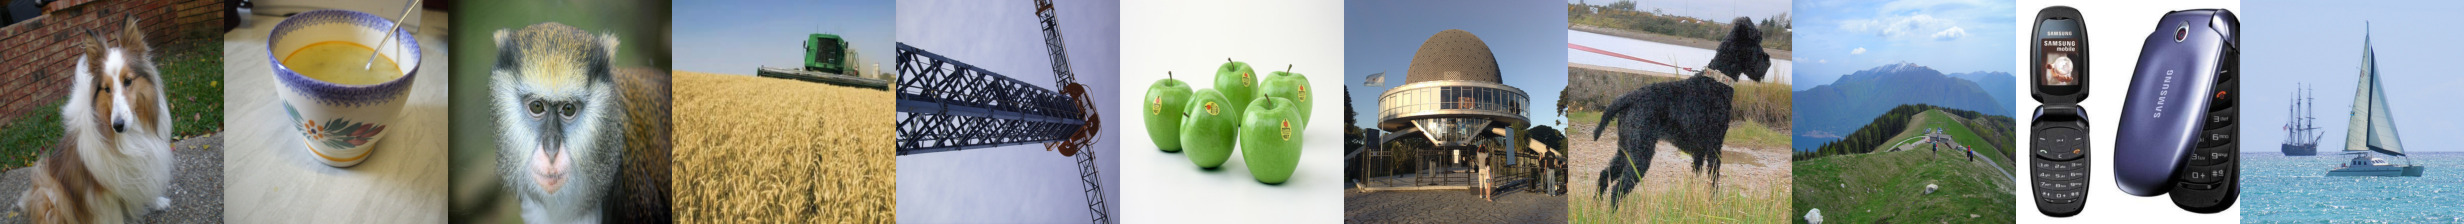
\includegraphics[width=\textwidth]{figs/contrast/contrast_tile0.jpg}}

\vspace{-.9\baselineskip}
\subfloat[DeePSiM inversion results \cite{dosovitskiy_2016_generating}.]{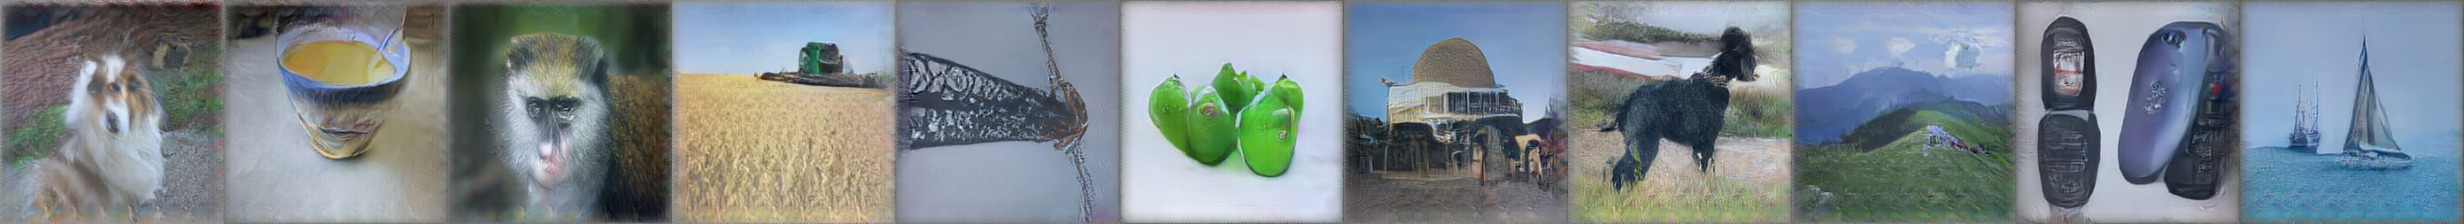
\includegraphics[width=\textwidth]{figs/contrast/contrast_tile1.jpg}}

\vspace{-.9\baselineskip}
\subfloat[RI results \cite{engstrom_2019_adversarial}.]{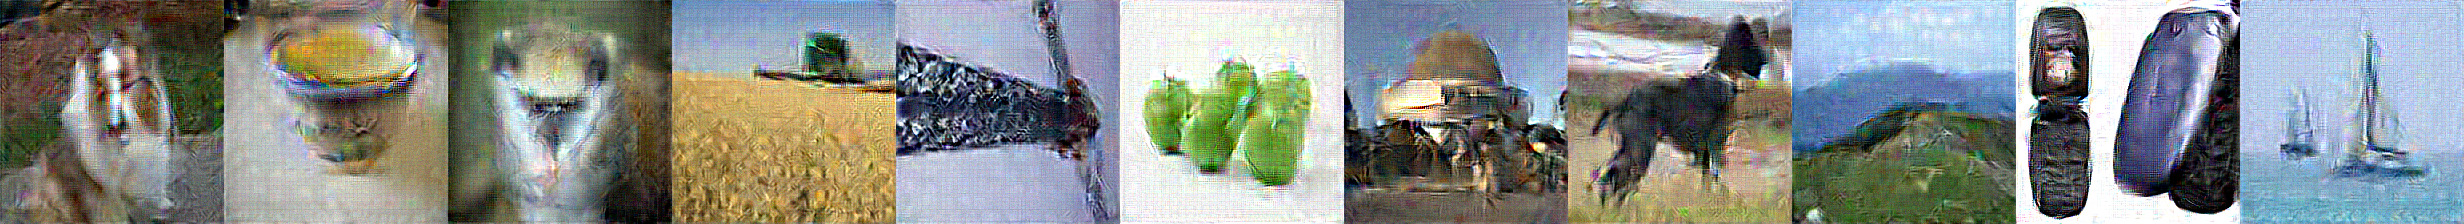
\includegraphics[width=\textwidth]{figs/contrast/contrast_tile2.jpg}}

\vspace{-.9\baselineskip}
\subfloat[Standard autoencoder.]{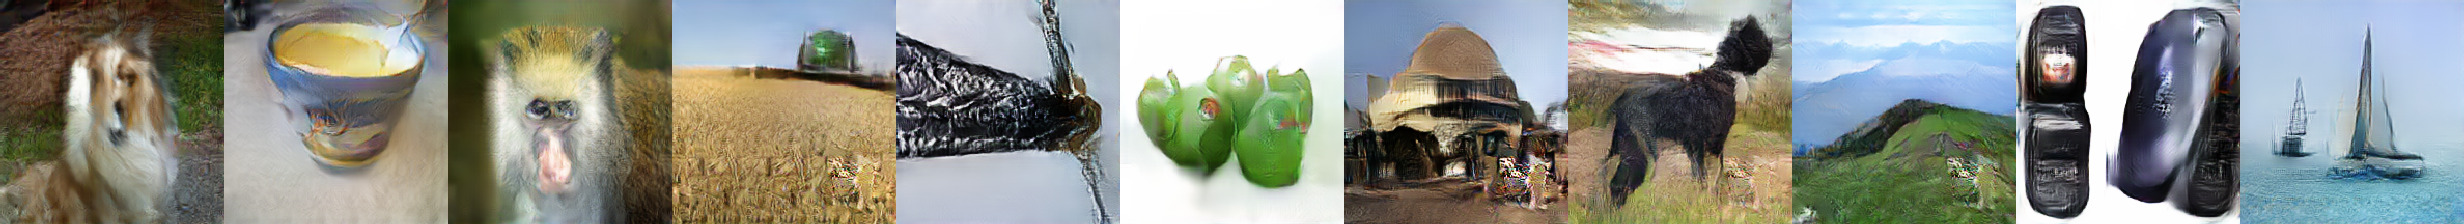
\includegraphics[width=\textwidth]{figs/contrast/contrast_tile3.jpg}}

\vspace{-.9\baselineskip}
\subfloat[Robust autoencoder (ours).]{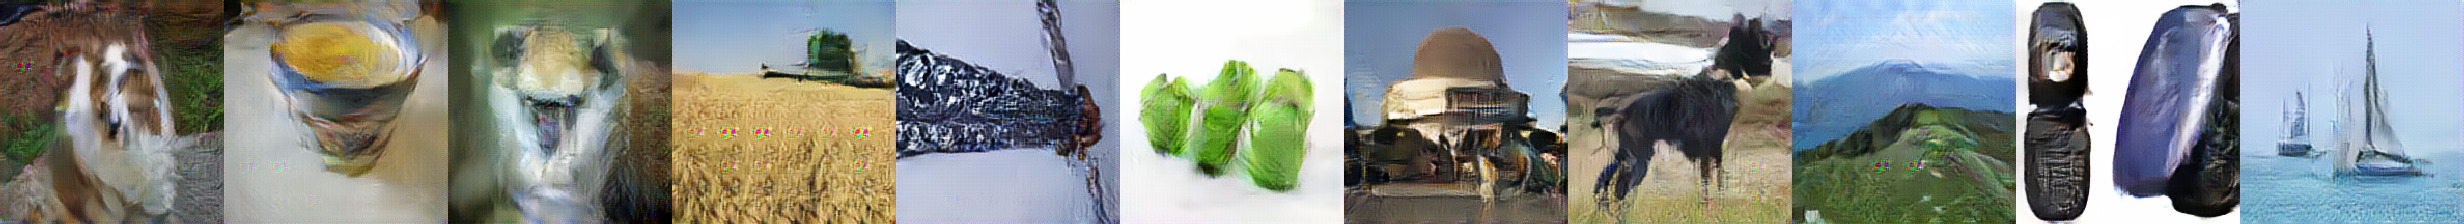
\includegraphics[width=\textwidth]{figs/contrast/contrast_tile4.jpg}}

\caption{Feature inversion accuracy contrast between our proposed model and alternative inversion methods.}
\label{fig:supp_contrast}
\end{figure*}


\section{Additional Results on Downstream Tasks}
\label{sec:supp_additional}
    \subsection{Style Transfer}
    \label{sec:supp_additional_st}
    \figref{fig:supp_st} shows additional stylization results obtained via the Universal Style Transfer algorithm using standard and AR AlexNet autoencoders. Qualitatively, the multi-level stylization approach used in our experiments show that AR representations allow a good texture transferring while better preserving the content image structure. Regardless the type of scene being stylized (\eg landscapes, portraits or single objects), aligning AR robust features allows to preserve sharp edges and alleviates the distortions generated by aligning standard features. Architecture details and training parameters for the style transfer experiments are covered in \secref{sec:supp_proposed_st}.
    \begin{figure}[t]
\begin{minipage}[t]{0.1\textwidth}
\centering\textbf{\scriptsize{Refs}}
\end{minipage}\begin{minipage}[t]{0.2\textwidth}
\centering \textbf{\scriptsize{Standard}}
\end{minipage}\begin{minipage}[t]{0.2\textwidth}
\centering \textbf{\scriptsize{AR (ours)}}
\end{minipage}\begin{minipage}[t]{0.1\textwidth}
\centering\textbf{\scriptsize{Refs}}
\end{minipage}\begin{minipage}[t]{0.2\textwidth}
\centering \textbf{\scriptsize{Standard}}
\end{minipage}\begin{minipage}[t]{0.2\textwidth}
\centering \textbf{\scriptsize{AR (ours)}}
\end{minipage}

\vspace{-0.9\baselineskip}
\subfloat[]{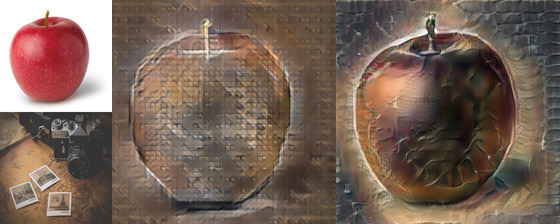
\includegraphics[width=0.5\textwidth]{figs/st/st_tile07.jpg}}
\subfloat[]{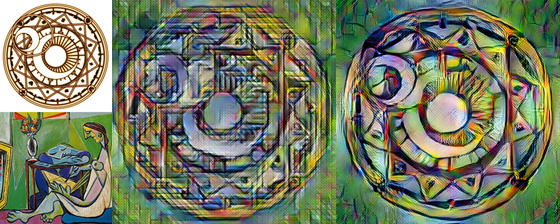
\includegraphics[width=0.5\textwidth]{figs/st/st_tile02.jpg}}

\vspace{-.9\baselineskip}
\subfloat[]{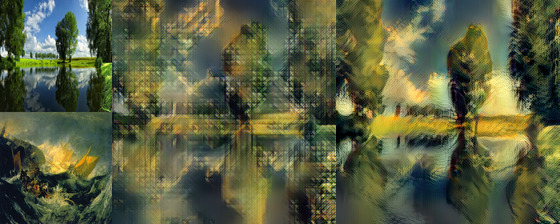
\includegraphics[width=0.5\textwidth]{figs/st/st_tile08.jpg}}
\subfloat[]{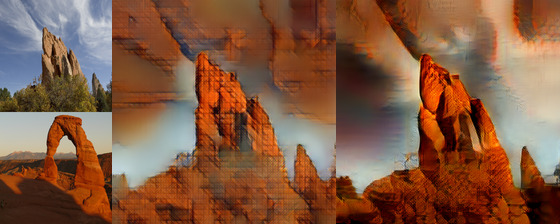
\includegraphics[width=0.5\textwidth]{figs/st/st_tile09.jpg}}

\vspace{-.9\baselineskip}
\subfloat[]{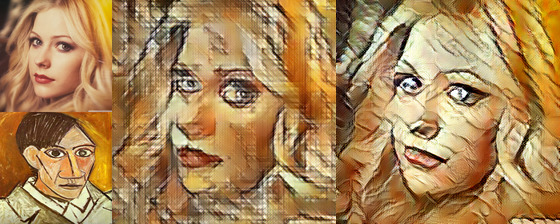
\includegraphics[width=0.5\textwidth]{figs/st/st_tile04.jpg}}
\subfloat[]{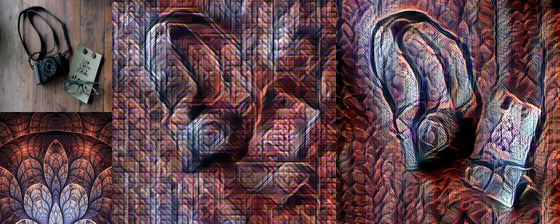
\includegraphics[width=0.5\textwidth]{figs/st/st_tile06.jpg}}

\vspace{-.9\baselineskip}
\subfloat[]{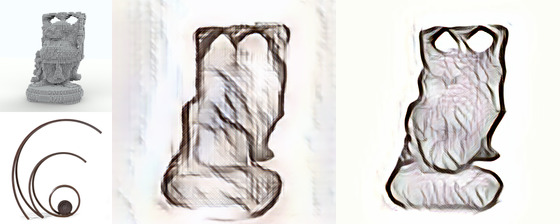
\includegraphics[width=0.5\textwidth]{figs/st/st_tile10.jpg}}
\subfloat[]{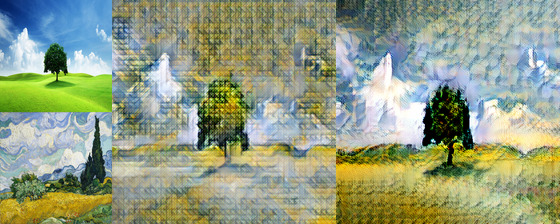
\includegraphics[width=0.5\textwidth]{figs/st/st_tile11.jpg}}
\vspace{-0.5\baselineskip}

\caption{Style transfer results using standard and robust AlexNet representations. Stylization obtained using the universal style transfer algorithm \cite{li_2017_universal}.}
\label{fig:supp_st}
\vspace{-0.8 cm}
\end{figure}


    \begin{figure*}[t]

\begin{minipage}{0.25\textwidth}
\centering\textbf{\colorbox{white}{\scalebox{.7}{Ground-truth}}}
\end{minipage}\begin{minipage}{0.25\textwidth}
\centering \textbf{\colorbox{white}{\scalebox{.7}{Noisy}}}
\end{minipage}\begin{minipage}{0.25\textwidth}
\centering \textbf{\colorbox{white}{\scalebox{.7}{Standard}}}
\end{minipage}\begin{minipage}{0.25\textwidth}
\centering\textbf{\colorbox{white}{\scalebox{.7}{Robust}}}
\end{minipage}

\vspace{-\baselineskip}
\subfloat{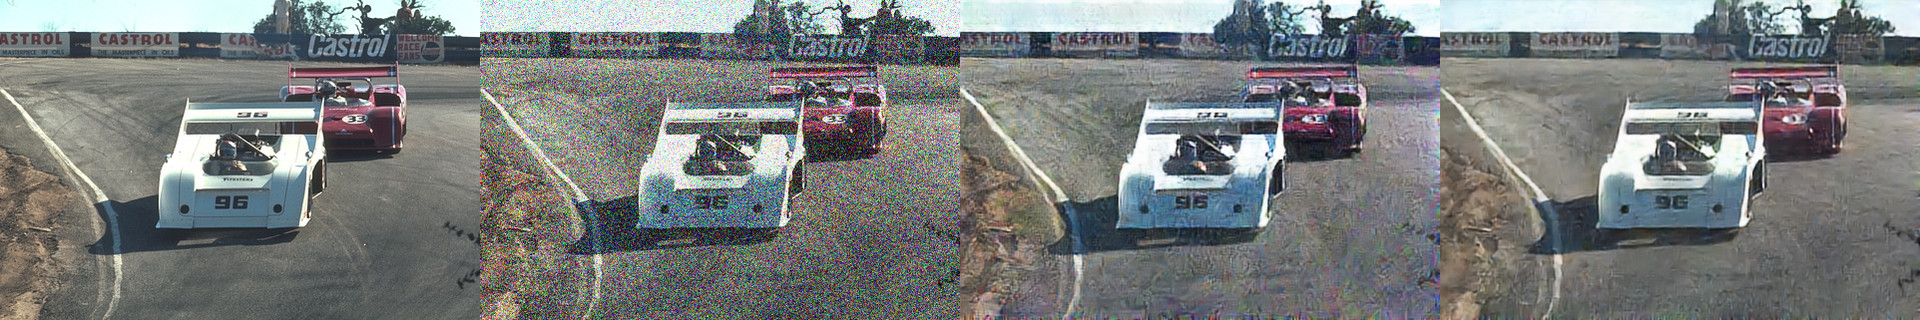
\includegraphics[width=\textwidth]{figs/denoising/cbsd68_tile5.jpg}}

\vspace{-0.8\baselineskip}
\subfloat{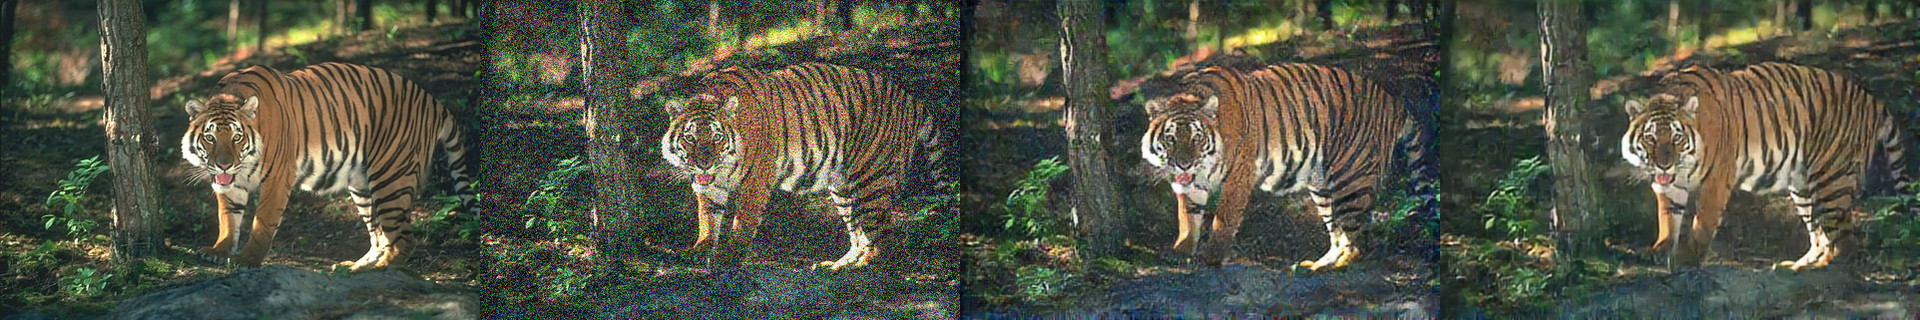
\includegraphics[width=\textwidth]{figs/denoising/cbsd68_tile14.jpg}}

\vspace{-0.8\baselineskip}
\subfloat{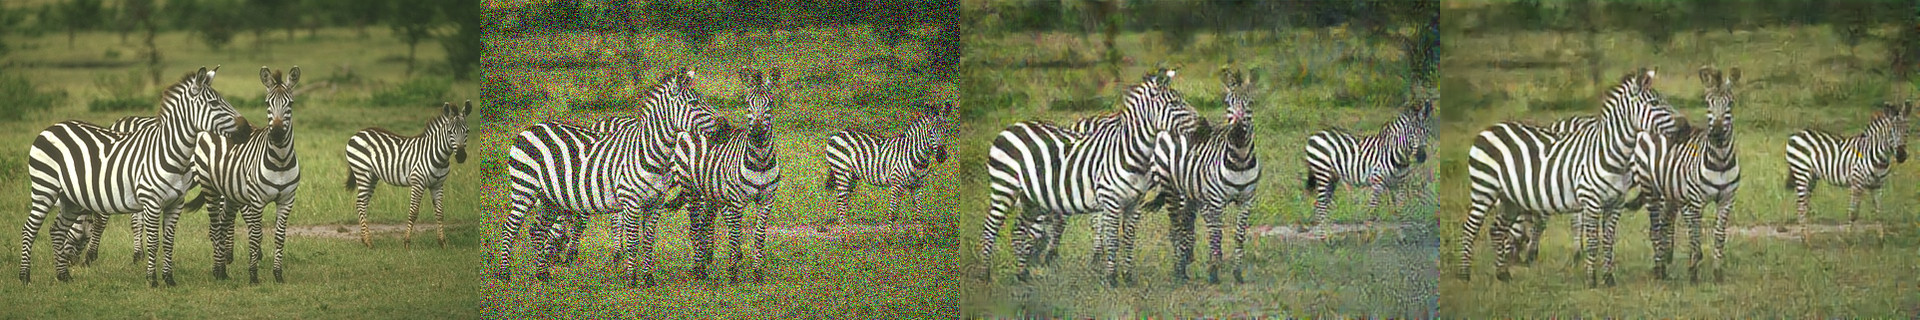
\includegraphics[width=\textwidth]{figs/denoising/cbsd68_tile52.jpg}}

\vspace{-0.8\baselineskip}
\subfloat{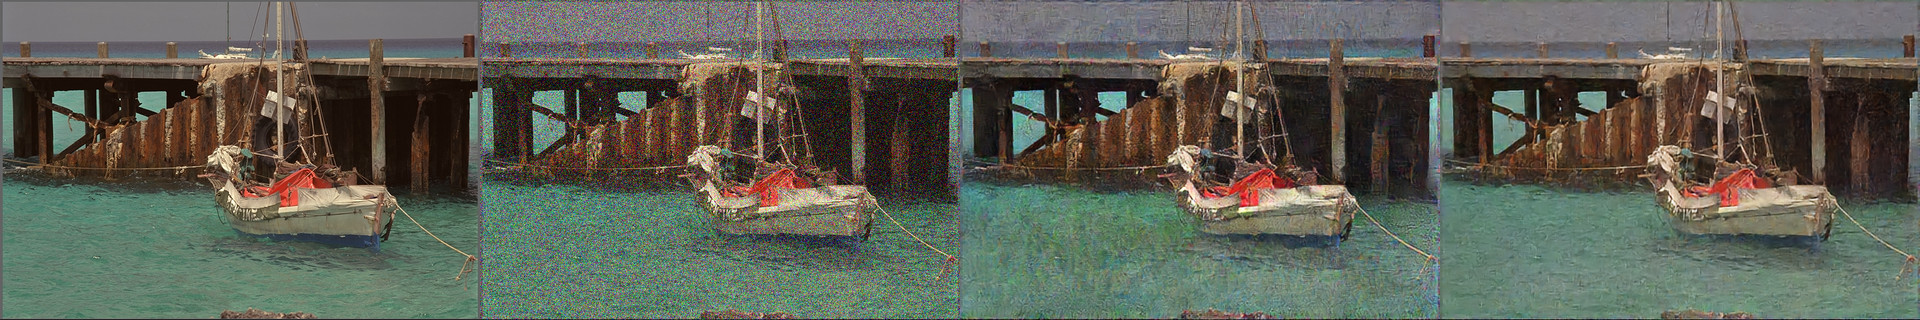
\includegraphics[width=\textwidth]{figs/denoising/kodak24_tile10.jpg}}

\vspace{-0.8\baselineskip}
\subfloat{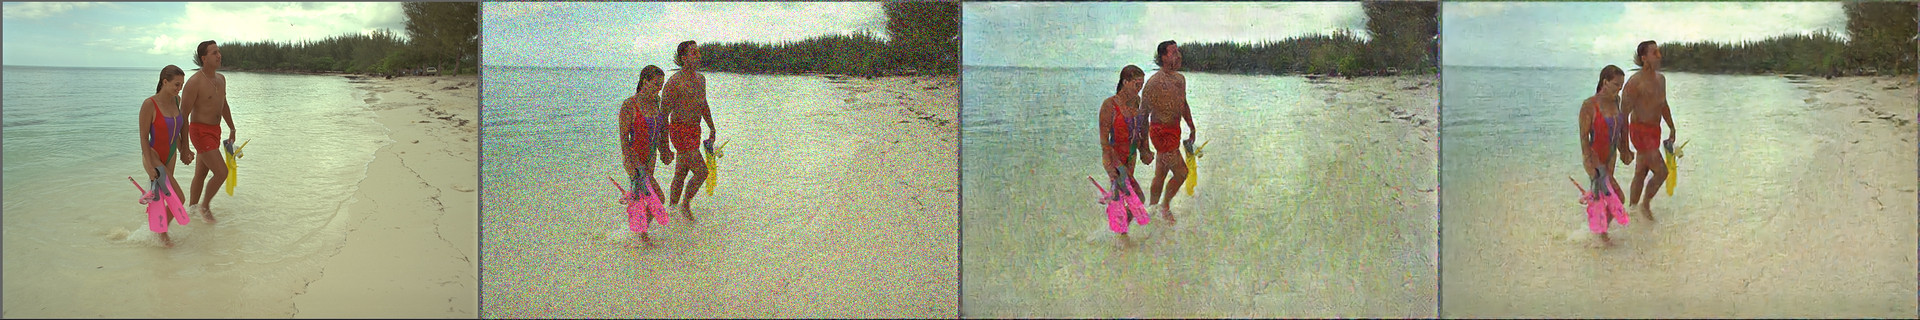
\includegraphics[width=\textwidth]{figs/denoising/kodak24_tile11.jpg}}

\vspace{-0.8\baselineskip}
\subfloat{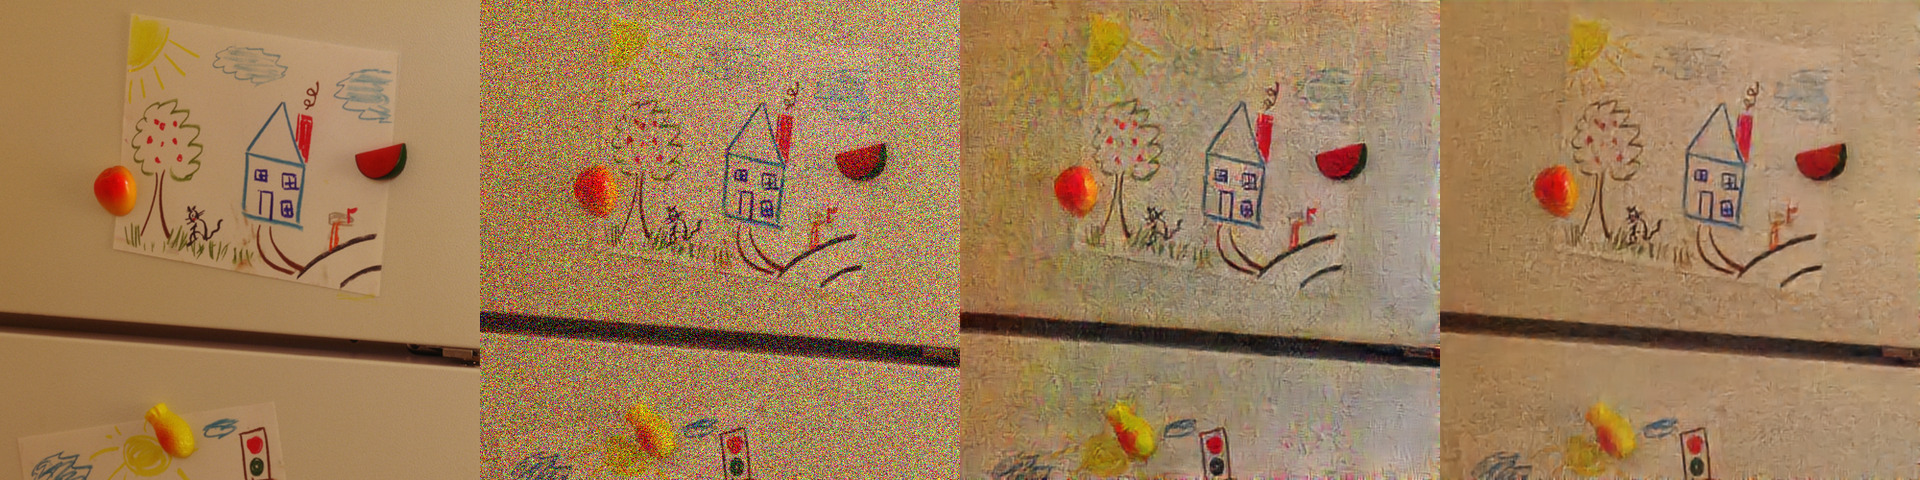
\includegraphics[width=\textwidth]{figs/denoising/mcmaster_tile4.jpg}}

\vspace{-0.8\baselineskip}
\subfloat{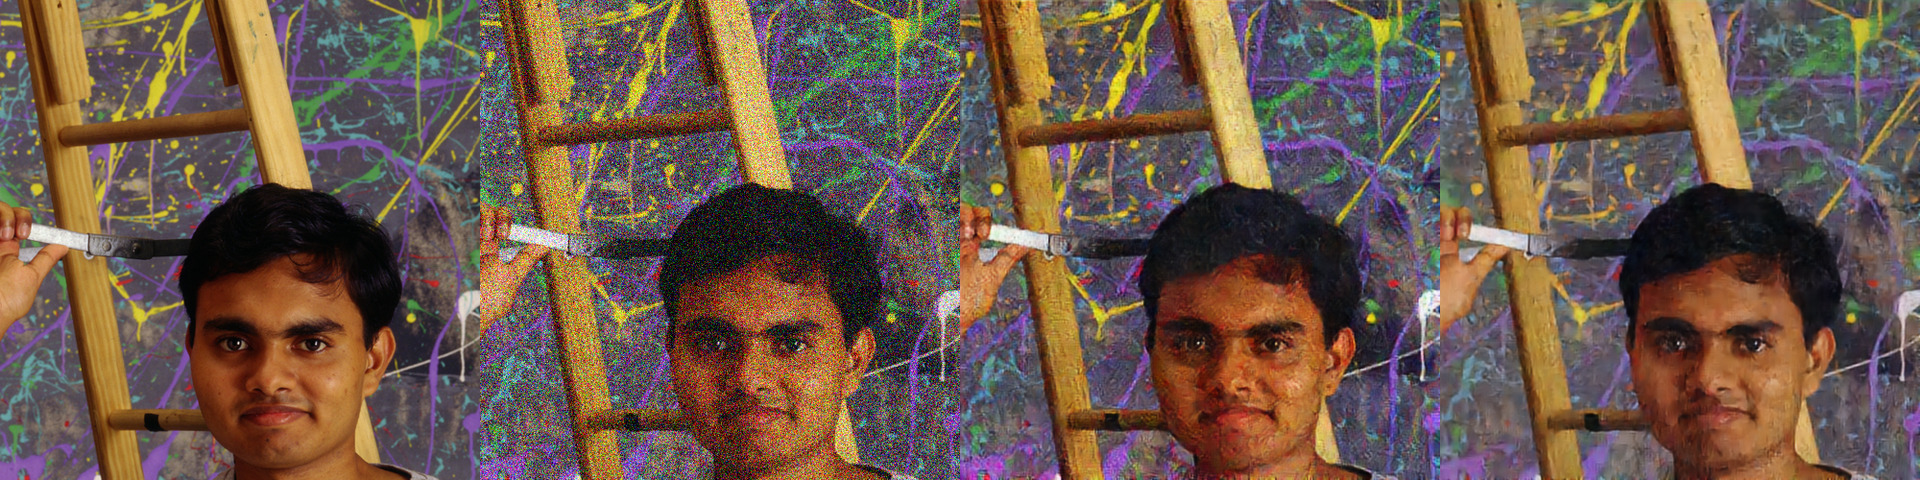
\includegraphics[width=\textwidth]{figs/denoising/mcmaster_tile14.jpg}}

\vspace{-0.3cm}
\caption{Image denoising results using standard and AR encoders (AlexNet) from the CBSD68 and Kodak24 sets. Samples corrupted by clipped white Gaussian noise $(\sigma= \frac{50}{255})$.}
\label{fig:supp_denoising}
\vspace{-0.6cm}
\end{figure*}

    \subsection{Image Denoising}
    \label{sec:supp_additional_denoising}
    \figref{fig:supp_denoising} shows additional denoising results using our standard and AR autoencoders for the CBSDS68, Kodak24 and McMaster datasets. As previously discussed, we leverage the low-level feature representations by adding skip connections to our proposed autoencoder. Low-level features complement the contracted feature map obtained from AlexNet \layer{conv5}, improving the detail preservation. This is observed in the results, both with standard and AR autoencoders.
    
    On the other hand, despite the effect of using skip connections, reconstructions from AR representations show a notorious improvement with respect to standard reconstructions. Specifically, by combining skip connections with the rich information already encapsulated in robust representations, results on all three datasets show a substantial denoising improvement.

\section{Implementation Details}\label{sec:supp_proposed_method}
    \subsection{Architecture and Training Details}
    \label{sec:supp_proposed}
    
    \textbf{Encoder.} For all downstream tasks, our adversarially robust AlexNet classifier was trained using PGD attacks \cite{madry_2018_towards}. The process was performed on ImageNet using stochastic gradient descent. The AR training parameters are as follows:
    \begin{itemize}
        \item Perturbation constraint: $\ell_{2}$ ball with $\varepsilon=3$
        \item PGD attack steps: $7$
        \item Step size: $0.5$
        \item Training epochs: $90$
    \end{itemize}
    
    On the other hand, the standard AlexNet classifier was trained using cross-entropy loss as optimization criteria. For both cases, the training parameters were the following:
    \begin{itemize}
        \item Initial learning rate: $0.1$
        \item Optimizer: Learn rate divided by a factor of $10$ every $30$ epochs.
        \item Batch size: $256$
    \end{itemize}

    Tested under AutoAttack ($\ell_{2}, \varepsilon=3$), our AR AlexNet obtains a $18.7\%$ top-1 robust accuracy, while our standard AlexNet classifier obtains a $0\%$ top-1 robust accuracy.
    
    AR training was performed using the \textit{Robustness} library \cite{robustness} on four Tesla V100 GPUs. Additional details about the model architecture and training parameters used for each experiment and downstream task are as follows.
    
    \textbf{Feature Inversion Experiments.} A fully convolutional architecture is used for the decoder or image generator. \tabref{tab:supp_generator01} describes the decoder architecture used to invert both standard and AR representations, where \texttt{conv2d} denotes a $2$D convolutional layer, \texttt{tconv2d} a $2$D transposed convolutional layer, \texttt{BN} batch normalization, \texttt{ReLU} the rectified linear unit operator and \texttt{tanh} the hyperbolic tangent operator.
    
    \begin{figure}[t]
\vspace{-1 cm}
\centering
\subfloat[]{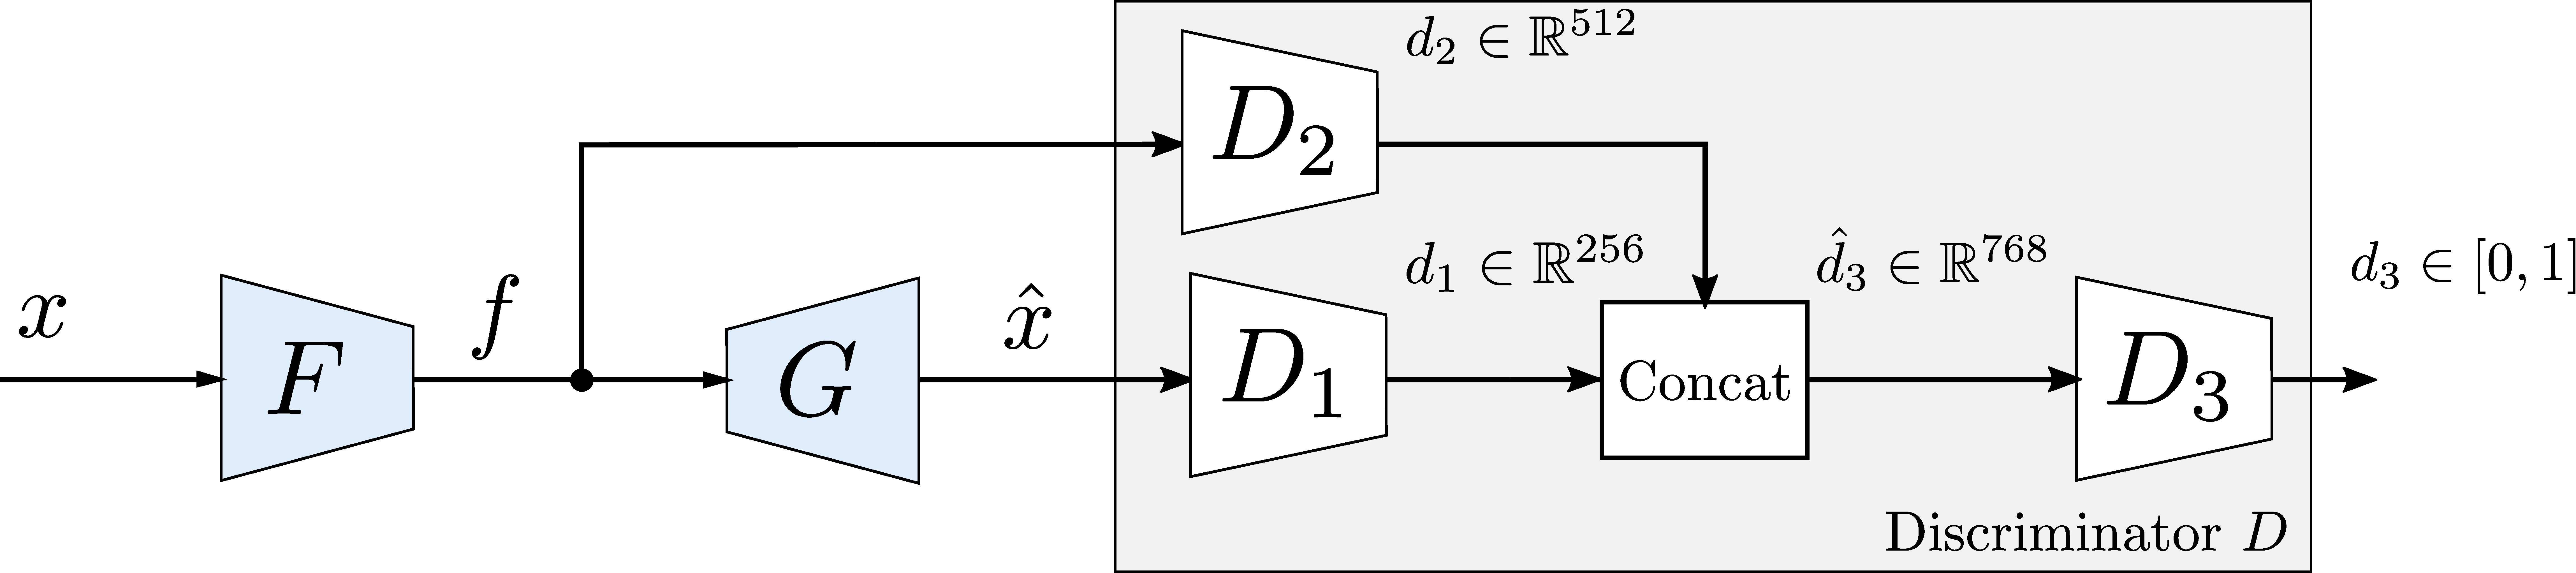
\includegraphics[width=0.9\textwidth]{figs/proposed/discriminator.pdf}}

\vspace{-0.3cm}
\caption{Discriminator model.}
\label{fig:supp_disc_diag}
\vspace{-0.6cm}
\end{figure}

    
    \tabref{tab:supp_discriminator01} shows the discriminator architecture, where \texttt{leakyReLU} corresponds to the leaky rectified linear unit, \texttt{linear} to a fully-connected layer, \texttt{apooling} to average pooling and \texttt{sigmoid} to the Sigmoid operator. Motivated by the architecture proposed by Dosovitskiy \& Brox \cite{dosovitskiy_2016_generating}, the discriminator takes as input both a real or fake image and its target \layer{conv5} feature map to compute the probability of the sample being real. \figref{fig:supp_disc_diag} shows the discriminator architecture.
    
    
    Standard and AR autoencoders were trained on ImageNet using $\ell_{1}$ pixel, feature and GAN losses using ADAM. In both cases, all convolutional and transposed convolutional layers are regularized using spectral normalization \cite{miyato_2018_spectral}. Training was performed using Pytorch-only code on two Tesla V100 GPUs.
    
    The loss weights and training setup for both standard and AR cases correspond to:
    \begin{itemize}
     \setlength\itemsep{0.1\baselineskip}
        \item Generator weights: $\lambda_{\text{pix}}=2\times 10^{-6}, \lambda_{\text{feat}}=1\times 10^{-2}, \lambda_{\text{GAN}}= 100$
        \item Discriminator weight: $\lambda_{\text{disc}}=2\times 10^{-6}$
        \item Training epochs: $90$
        \item Generator initial learning rate: $3\times 10^{-4}$ (divided by a factor of $10$ every $30$ epochs).
        \item Discriminator initial learning rate: $12\times 10^{-4}$ (divided by a factor of $10$ every $30$ epochs).
        \item LeakyReLU factor: $0.2$
        \item ADAM $\beta\in [0, 0.9]$
        \item Batch size: $128$
    \end{itemize}
    
    \begin{table*}[t]
\begin{center}
\resizebox{0.9\textwidth}{!}{
\begin{tabular}{c|c|c|c|c|c|c|c|c|c}
\specialrule{.15em}{.05em}{.05em} 
\makecell{Layer}
& \makecell{Layer Type}
& \makecell{Kernel\\ Size}
& \makecell{Bias}
& \makecell{Stride}
& \makecell{Pad}
& \makecell{Input\\ Size}
& \makecell{Output\\ Size}
& \makecell{Input\\ Channels}
& \makecell{Output\\ Channels} \\
\midrule
1a & conv2d + BN + ReLU & $3\times 3$ & \xmark & $1$ & $1$ & $6\times 6$ & $6\times 6$ & $256$ & $256$ \\
\midrule
2a & tconv2d + BN + ReLU & $4\times 4$ & \xmark & $1$ & $1$ & $6\times 6$ & $7\times 7$ & $256$ & $256$ \\
2b & conv2d + BN + ReLU & $3\times 3$ & \xmark & $1$ & $1$ & $7\times 7$ & $7\times 7$ & $256$ & $256$ \\
\midrule
3a & tconv2d + BN + ReLU & $4\times 4$ & \xmark & $2$ & $1$ & $7\times 7$ & $14\times 14$ & $256$ & $256$ \\
3b & conv2d + BN + ReLU & $3\times 3$ & \xmark & $1$ & $1$ & $14\times 14$ & $14\times 14$ & $256$ & $256$ \\
\midrule
4a & tconv2d + BN + ReLU & $4\times 4$ & \xmark & $2$ & $1$ & $14\times 14$ & $28\times 28$ & $256$ & $256$ \\
4b & conv2d + BN + ReLU & $3\times 3$ & \xmark & $1$ & $1$ & $28\times 28$ & $28\times 28$ & $256$ & $128$ \\
\midrule
5a & tconv2d + BN + ReLU & $4\times 4$ & \xmark & $2$ & $1$ & $28\times 28$ & $56\times 56$ & $128$ & $128$ \\
5b & conv2d + BN + ReLU & $3\times 3$ & \xmark & $1$ & $1$ & $56\times 56$ & $56\times 56$ & $128$ & $64$ \\
\midrule
6a & tconv2d + BN + ReLU & $4\times 4$ & \xmark & $2$ & $1$ & $56\times 56$ & $112\times 112$ & $64$ & $64$ \\
6b & conv2d + BN + ReLU & $3\times 3$ & \xmark & $1$ & $1$ & $112\times 112$ & $112\times 112$ & $64$ & $32$ \\
\midrule
7a & tconv2d + BN + ReLU & $4\times 4$ & \xmark & $2$ & $1$ & $112\times 112$ & $224\times 224$ & $32$ & $32$ \\
7b & conv2d + BN + ReLU & $3\times 3$ & \xmark & $1$ & $1$ & $224\times 224$ & $224\times 224$ & $32$ & $3$ \\
7c & conv2d + tanh & $3\times 3$ & \cmark & $1$ & $1$ & $224\times 224$ & $224\times 224$ & $3$ & $3$\\
\specialrule{.15em}{.05em}{.05em}
\end{tabular}}
\end{center}
\vspace{-0.3 cm}
\caption{\label{tab:supp_generator01} Generator architecture used for feature inversion.}
\vspace{-0.6 cm}
\end{table*}

    \begin{table*}[t]
\begin{center}
\resizebox{0.9\textwidth}{!}{
\begin{tabular}{c|c|c|c|c|c|c|c|c|c}
\specialrule{.15em}{.05em}{.05em} 
\makecell{Layer}
& \makecell{Layer Type}
& \makecell{Kernel\\ Size}
& \makecell{Bias}
& \makecell{Stride}
& \makecell{Pad}
& \makecell{Input\\ Size}
& \makecell{Output\\ Size}
& \makecell{Input\\ Channels}
& \makecell{Output\\ Channels} \\
\specialrule{.15em}{.05em}{.05em}
\multicolumn{10}{c}{Feature Extractor 1 ($D_{1}$)}\\
\midrule
1a & conv2d + ReLU & $3\times 3$ & \cmark & $4$ & $1$ & $256\times 256$ & $56\times 56$ & $3$ & $32$ \\
\midrule
2a & conv2d + ReLU & $5\times 5$ & \cmark & $1$ & $1$ & $56\times 56$ & $52\times 52$ & $32$ & $64$ \\
2b & conv2d + ReLU & $3\times 3$ & \cmark & $2$ & $1$ & $52\times 52$ & $23\times 23$ & $64$ & $128$ \\
\midrule
3a & conv2d + ReLU & $3\times 3$ & \cmark & $1$ & $1$ & $23\times 23$ & $21\times 21$ & $128$ & $256$ \\
3b & conv2d + ReLU & $3\times 3$ & \cmark & $2$ & $1$ & $21\times 21$ & $11\times 11$ & $256$ & $256$ \\
\midrule
4 & ave. pooling & $11 \times 11$ & $-$ & $-$ & $-$ & $11\times 11$ & $1 \times 1$ & $256$ & $256$\\
\specialrule{.15em}{.05em}{.05em}
\multicolumn{10}{c}{Classifier 1 ($D_{2}$)}\\
\midrule
4a & Linear + ReLU & $-$ & \cmark & $-$ & $1$ & $9216$ & $1024$ & $-$ & $-$ \\
4b & Linear + ReLU & $-$ & \cmark & $-$ & $1$ & $1024$ & $512$ & $-$ & $-$ \\
\specialrule{.15em}{.05em}{.05em}
\multicolumn{10}{c}{Classifier 2 ($D_{3}$)}\\
\midrule
5a & Linear + ReLU & $-$ & \cmark & $-$ & $1$ & $768$ & $512$ & $-$ & $-$ \\
5b & Linear + Sigmoid & $-$ & \cmark & $-$ & $1$ & $512$ & $1$ & $-$ & $-$ \\
\specialrule{.15em}{.05em}{.05em}
\end{tabular}}
\end{center}
\vspace{-0.3 cm}
\caption{\label{tab:supp_discriminator01} Discriminator architecture used for feature inversion.}
\vspace{-0.6 cm}
\end{table*}

       
    \subsection{Style Transfer}
    \label{sec:supp_proposed_st}
    
    While, for standard and AR scenarios, the autoencoder associated to \layer{conv5} corresponds to the model described in \secref{sec:supp_proposed}, those associated to \layer{conv1} and \layer{conv2} use Nearest neighbor interpolation instead of transposed convolution layers to improve the reconstruction accuracy and to avoid the checkerboard effect generated by transposed convolutional layers. \tabref{tab:supp_st01}, and \tabref{tab:supp_st02} describe their architecture details.
    
    All generators were fully-trained on ImageNet using Pytorch-only code on two Tesla V100 GPUs. The regularization parameters and training setup for both cases are as follows:
    \begin{itemize}
     \setlength\itemsep{0.1\baselineskip}
        \item Standard generator weights: $\lambda_{\text{pix}}=2\times 10^{-4}, \lambda_{\text{feat}}=1\times 10^{-2}$.
        \item AR generator weights: $\lambda_{\text{pix}}=2\times 10^{-6}, \lambda_{\text{feat}}=1\times 10^{-2}$.
        \item Training epochs: $90$.
        \item Generator initial learning rate: $3\times 10^{-4}$ (divided by a factor of $10$ every $30$ epochs).
        \item ADAM $\beta\in [0, 0.9]$.
        \item Batch size: $128$.
    \end{itemize}
    
    \begin{table*}[t]
\begin{center}
\resizebox{0.9\textwidth}{!}{
\begin{tabular}{c|c|c|c|c|c|c|c|c|c}
\specialrule{.15em}{.05em}{.05em} 
\makecell{Layer}
& \makecell{Layer Type}
& \makecell{Kernel\\ Size}
& \makecell{Bias}
& \makecell{Stride}
& \makecell{Pad}
& \makecell{Input\\ Size}
& \makecell{Output\\ Size}
& \makecell{Input\\ Channels}
& \makecell{Output\\ Channels} \\
\midrule
1a & conv2d + BN + ReLU & $3\times 3$ & \xmark & $1$ & $1$ & $27\times 27$ & $27\times 27$ & $64$ & $64$ \\
\midrule
2a & tconv2d + BN + ReLU & $4\times 4$ & \xmark & $1$ & $1$ & $27\times 27$ & $28\times 28$ & $64$ & $64$ \\
2b & conv2d + BN + ReLU & $3\times 3$ & \xmark & $1$ & $1$ & $28\times 28$ & $28\times 28$ & $64$ & $64$ \\
\midrule
3a & NN interpolation & $-$ & $-$ & $2$ & $-$ & $28\times 28$ & $56\times 56$ & $64$ & $64$ \\
3b & conv2d + BN + ReLU & $3\times 3$ & \xmark & $1$ & $1$ & $56\times 56$ & $56\times 56$ & $64$ & $64$ \\
3c & conv2d + BN + ReLU & $3\times 3$ & \xmark & $1$ & $1$ & $56\times 56$ & $56\times 56$ & $64$ & $32$ \\
\midrule
4a & NN interpolation & $-$ & $-$ & $2$ & $-$ & $56\times 56$ & $112\times 112$ & $32$ & $32$ \\
4b & conv2d + BN + ReLU & $3\times 3$ & \xmark & $1$ & $1$ & $112 \times 112$ & $112\times 112$ & $32$ & $32$ \\
\midrule
5a & NN interpolation & $-$ & $-$ & $2$ & $-$ & $112\times 112$ & $224\times 224$ & $32$ & $32$ \\
5b & conv2d + BN + ReLU & $3\times 3$ & \xmark & $1$ & $1$ & $224\times 224$ & $224\times 224$ & $32$ & $16$ \\
5c & conv2d + BN + ReLU & $3\times 3$ & \xmark & $1$ & $1$ & $224\times 224$ & $224\times 224$ & $16$ & $3$ \\
5d & conv2d + tanh & $3\times 3$ & \cmark & $1$ & $1$ & $224\times 224$ & $224\times 224$ & $3$ & $3$\\
\specialrule{.15em}{.05em}{.05em}
\end{tabular}}
\end{center}
\vspace{-0.3 cm}
\caption{\label{tab:supp_st01} \layer{Conv1} generator architecture used for style transfer.}
\vspace{-0.6 cm}
\end{table*}

    \begin{table*}[t]
\begin{center}
\resizebox{0.9\textwidth}{!}{
\begin{tabular}{c|c|c|c|c|c|c|c|c|c}
\specialrule{.15em}{.05em}{.05em} 
\makecell{Layer}
& \makecell{Layer Type}
& \makecell{Kernel\\ Size}
& \makecell{Bias}
& \makecell{Stride}
& \makecell{Pad}
& \makecell{Input\\ Size}
& \makecell{Output\\ Size}
& \makecell{Input\\ Channels}
& \makecell{Output\\ Channels} \\
\midrule
1a & conv2d + BN + ReLU & $3\times 3$ & \xmark & $1$ & $1$ & $13\times 13$ & $13\times 13$ & $192$ & $192$ \\
\midrule
2a & tconv2d + BN + ReLU & $4\times 4$ & \xmark & $1$ & $1$ & $13\times 13$ & $14\times 14$ & $192$ & $192$ \\
2b & conv2d + BN + ReLU & $3\times 3$ & \xmark & $1$ & $1$ & $14\times 14$ & $14\times 14$ & $192$ & $96$ \\
\midrule
3a & NN interpolation & $-$ & $-$ & $2$ & $-$ & $14\times 14$ & $28\times 28$ & $96$ & $96$ \\
3b & conv2d + BN + ReLU & $3\times 3$ & \xmark & $1$ & $1$ & $28\times 28$ & $28\times 28$ & $96$ & $96$ \\
3c & conv2d + BN + ReLU & $3\times 3$ & \xmark & $1$ & $1$ & $28\times 28$ & $28\times 28$ & $96$ & $64$ \\
\midrule
4a & NN interpolation & $-$ & $-$ & $2$ & $-$ & $28\times 28$ & $56\times 56$ & $64$ & $64$ \\
4b & conv2d + BN + ReLU & $3\times 3$ & \xmark & $1$ & $1$ & $56 \times 56$ & $56\times 56$ & $64$ & $64$ \\
\midrule
5a & NN interpolation & $-$ & $-$ & $2$ & $-$ & $56\times 56$ & $112\times 112$ & $64$ & $64$ \\
5b & conv2d + BN + ReLU & $3\times 3$ & \xmark & $1$ & $1$ & $112\times 112$ & $112\times 112$ & $64$ & $64$ \\
\midrule
6a & NN interpolation & $-$ & $-$ & $2$ & $-$ & $112\times 112$ & $224\times 224$ & $64$ & $64$ \\
6b & conv2d + BN + ReLU & $3\times 3$ & \xmark & $1$ & $1$ & $224\times 224$ & $224\times 224$ & $64$ & $32$ \\
6c & conv2d + BN + ReLU & $3\times 3$ & \xmark & $1$ & $1$ & $224\times 224$ & $224\times 224$ & $32$ & $3$ \\
6d & conv2d + tanh & $3\times 3$ & \cmark & $1$ & $1$ & $224\times 224$ & $224\times 224$ & $3$ & $3$\\
\specialrule{.15em}{.05em}{.05em}
\end{tabular}}
\end{center}
\vspace{-0.3 cm}
\caption{\label{tab:supp_st02} \layer{Conv2} generator architecture used for style transfer.}
\vspace{-0.6 cm}
\end{table*}

    
    \subsection{Image Denoising}
    \label{sec:supp_proposed_denoising}
   
    Our image denoising model consists of standard and AR autoencoders equipped with skip connections to better preserve image details. \figref{fig:supp_den_diag} illustrates the proposed denoising model, where skip connections follow the Wavelet Pooling approach \cite{yoo_2019_photorealistic}. \tabref{tab:supp_den_enc} and \tabref{tab:supp_den_dec} include additional encoder and decoder architecture details, respectively.
    \begin{figure}[t]
\vspace{-1 cm}
\centering
\subfloat[Skip connected AlexNet encoder]{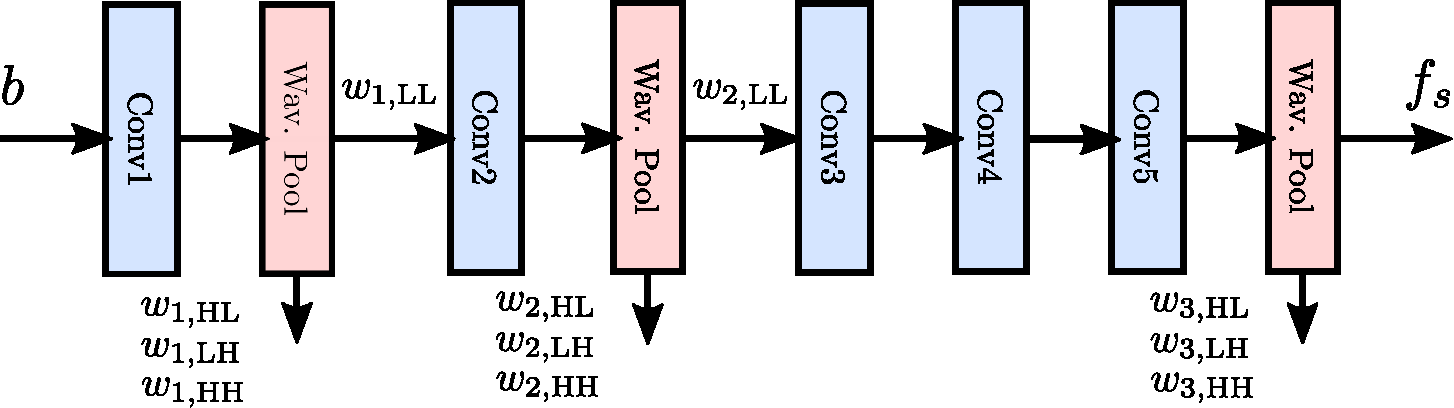
\includegraphics[height=0.09\textheight]{figs/proposed/den_enc.pdf}}

\subfloat[Skip connected AlexNet decoder]{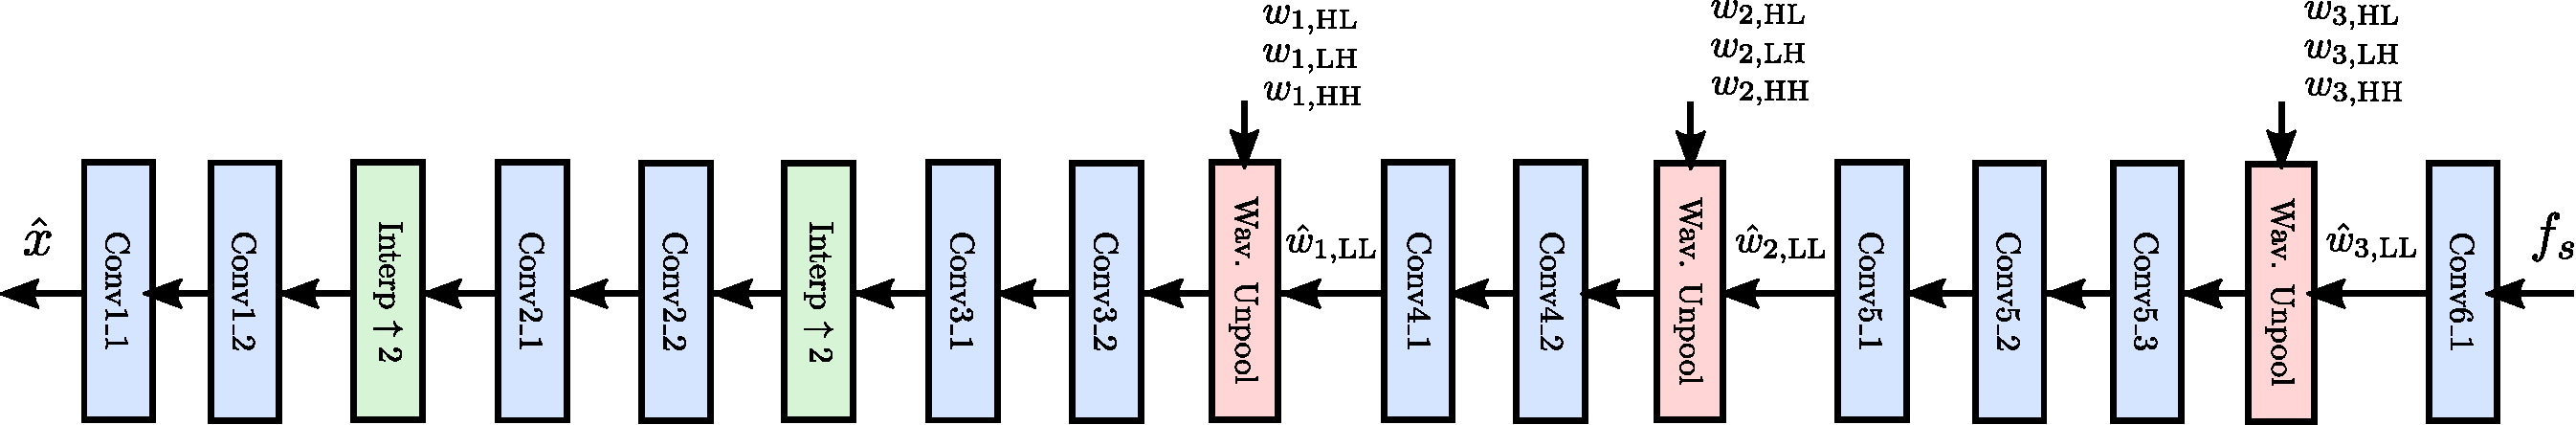
\includegraphics[width=1\textwidth]{figs/proposed/den_dec.pdf}}

\vspace{-0.3cm}
\caption{Proposed denoising autoencoder including skip connections.}
\label{fig:supp_den_diag}
\vspace{-0.6cm}
\end{figure}

    
    Encoder pooling layers are replaced by Haar wavelet analysis operators, generating an approximation component, denoted as $\{w_{k, \text{LL}}\}$, and three detail components, denoted as $\{w_{k, \text{LH}}, w_{k, \text{HL}}, w_{k, \text{HH}}\}$, where $k$ corresponds to the pooling level. While the approximation (low-frequency) component is passed to the next encoding layer, details are skip-connected to their corresponding stages in the decoder. Following this, transposed convolutional layers in the decoder are replaced by unpooling layers (Haar wavelet synthesis operators), reconstructing a signal with well-preserved details at each level and improving reconstruction.
    
    In contrast to the AlexNet architecture, all convolutional layers on the decoder use kernels of size $3 \times 3$. Also, given the striding factor of the first two AlexNet convolutional layers, two additional interpolation layers of striding factor $2$ are used to recover the original input size ($224 \times 224$).
    
    Standard and AR robust generators were trained using exclusively $\ell_{1}$ pixel and feature losses. Training was performed on ImageNet using Pytorch-only code on four Tesla V100 GPUs. Generator loss weights and training parameters for both cases correspond to:
    \begin{itemize}
     \setlength\itemsep{0.1\baselineskip}
        \item Generator weights: $\lambda_{\text{pix}}=2\times 10^{-6}, \lambda_{\text{feat}}=1\times 10^{-2}$.
        \item Training epochs: $90$.
        \item Generator initial learning rate: $3\times 10^{-4}$ (divided by a factor of $10$ every $30$ epochs).
        \item ADAM $\beta\in [0, 0.9]$.
        \item Batch size: $128$.
    \end{itemize}
    \begin{table*}[t]
\begin{center}
\resizebox{0.9\textwidth}{!}{
\begin{tabular}{c|c|c|c|c|c|c|c|c|c}
\specialrule{.15em}{.05em}{.05em} 
\makecell{Layer}
& \makecell{Layer Type}
& \makecell{Kernel\\ Size}
& \makecell{Bias}
& \makecell{Stride}
& \makecell{Pad}
& \makecell{Input\\ Size}
& \makecell{Output\\ Size}
& \makecell{Input\\ Channels}
& \makecell{Output\\ Channels} \\
\midrule
1a & conv2d + ReLU & $11\times 11$ & \cmark & $4$ & $2$ & $224\times 224$ & $55\times 55$ & $3$ & $64$ \\
\midrule
2a & Wavelet pooling & $-$ & $-$ & $2$ & $-$ & $55\times 55$ & $27\times 27$ & $64$ & $64$ \\
2b & conv2d + ReLU & $5\times 5$ & \cmark & $1$ & $2$ & $27\times 27$ & $27\times 27$ & $64$ & $192$ \\
\midrule
3a & Wavelet pooling & $-$ & $-$ & $2$ & $-$ & $27\times 27$ & $13\times 13$ & $192$ & $192$ \\
3b & conv2d + ReLU & $3\times 3$ & \cmark & $1$ & $1$ & $13\times 13$ & $13\times 13$ & $192$ & $384$ \\
3c & conv2d + ReLU & $3\times 3$ & \cmark & $1$ & $1$ & $13\times 13$ & $13\times 13$ & $384$ & $256$ \\
3c & conv2d + ReLU & $3\times 3$ & \cmark & $1$ & $1$ & $13\times 13$ & $13\times 13$ & $256$ & $256$ \\
\midrule
4a & Wavelet pooling & $-$ & $-$ & $2$ & $-$ & $13\times 13$ & $6\times 6$ & $256$ & $256$ \\
\specialrule{.15em}{.05em}{.05em}
\end{tabular}}
\end{center}
\vspace{-0.3 cm}
\caption{\label{tab:supp_den_enc} Encoder architecture used for image denoising.}
\vspace{-0.6 cm}
\end{table*}

    \begin{table*}[t]
\begin{center}
\resizebox{0.9\textwidth}{!}{
\begin{tabular}{c|c|c|c|c|c|c|c|c|c}
\specialrule{.15em}{.05em}{.05em} 

& \makecell{Layer Type}
& \makecell{Kernel\\ Size}
& \makecell{Bias}
& \makecell{Stride}
& \makecell{Pad}
& \makecell{Input\\ Size}
& \makecell{Output\\ Size}
& \makecell{Input\\ Channels}
& \makecell{Output\\ Channels} \\
\midrule
1a & conv2d + BN + ReLU & $3\times 3$ & \xmark & $1$ & $1$ & $6\times 6$ & $6\times 6$ & $256$ & $256$ \\
\midrule
2a & Wavelet unpooling & $-$ & $-$ & $2$ & $-$ & $6\times 6$ & $12\times 12$ & $256$ & $256$ \\
2b & conv2d + BN + ReLU & $3\times 3$ & \xmark & $1$ & $1$ & $12\times 12$ & $12\times 12$ & $256$ & $256$ \\
2c & Reflection padding & $-$ & $-$ & $-$ & $-$ & $12\times 12$ & $13\times 13$ & $256$ & $256$ \\
2d & conv2d + BN + ReLU & $3\times 3$ & \xmark & $1$ & $1$ & $13\times 13$ & $13\times 13$ & $256$ & $256$ \\
2e & conv2d + BN + ReLU & $3\times 3$ & \xmark & $1$ & $1$ & $13\times 13$ & $13\times 13$ & $256$ & $192$ \\
\midrule
3a & Wavelet unpooling & $-$ & $-$ & $2$ & $-$ & $13\times 13$ & $26\times 26$ & $192$ & $192$ \\
3b & Reflection padding & $-$ & $-$ & $-$ & $-$ & $26\times 26$ & $27\times 27$ & $192$ & $192$ \\
3c & conv2d + BN + ReLU & $3\times 3$ & \xmark & $1$ & $1$ & $27\times 27$ & $27\times 27$ & $192$ & $128$ \\
3d & conv2d + BN + ReLU & $3\times 3$ & \xmark & $1$ & $1$ & $27\times 27$ & $27\times 27$ & $128$ & $64$ \\
\midrule
4a & Wavelet unpooling & $-$ & $-$ & $2$ & $-$ & $27\times 27$ & $55\times 55$ & $64$ & $64$ \\
4b & Reflection padding & $-$ & $-$ & $-$ & $-$ & $55\times 55$ & $56\times 56$ & $64$ & $64$ \\
4c & conv2d + BN + ReLU & $3\times 3$ & \xmark & $1$ & $1$ & $56 \times 56$ & $56\times 56$ & $64$ & $64$ \\
\midrule
5a & NN interpolation & $-$ & $-$ & $2$ & $-$ & $56\times 56$ & $112\times 112$ & $64$ & $64$ \\
5b & conv2d + BN + ReLU & $3\times 3$ & \xmark & $1$ & $1$ & $112 \times 112$ & $112\times 112$ & $64$ & $32$ \\
5c & conv2d + BN + ReLU & $3\times 3$ & \xmark & $1$ & $1$ & $112 \times 112$ & $112\times 112$ & $32$ & $32$ \\
\midrule
6a & NN interpolation & $-$ & $-$ & $2$ & $-$ & $112\times 112$ & $224\times 224$ & $32$ & $32$ \\
6b & conv2d + BN + ReLU & $3\times 3$ & \xmark & $1$ & $1$ & $224\times 224$ & $224\times 224$ & $32$ & $3$ \\
6c & conv2d + BN + ReLU & $3\times 3$ & \xmark & $1$ & $1$ & $224\times 224$ & $224\times 224$ & $3$ & $3$ \\
6d & conv2d + tanh & $3\times 3$ & \cmark & $1$ & $1$ & $224\times 224$ & $224\times 224$ & $3$ & $3$\\
\specialrule{.15em}{.05em}{.05em}
\end{tabular}}
\end{center}
\caption{\label{tab:supp_den_dec} Decoder architecture used for image denoising.}
\end{table*}

